\documentclass[12pt,letterpaper]{article}
\usepackage[bottom=1in, top=1in]{geometry}
\usepackage[intlimits]{amsmath}
\usepackage{mathtools} % for splitfrac
\usepackage[utf8]{inputenc}
\DeclareUnicodeCharacter{2212}{-}
\usepackage{amsfonts,amssymb}
\DeclareSymbolFontAlphabet{\mathbb}{AMSb}
\usepackage{slashed}
\usepackage{textcomp}

\usepackage{float}
\usepackage[]{caption,subcaption}
\setcaptionmargin{0.5in}

\usepackage{fancyhdr}
%\usepackage{fancyheadings} % what does this do?
\usepackage{fancybox}

\usepackage{ifthen}
\usepackage{lscape,afterpage}
\usepackage{xspace}

\usepackage{siunitx}
\sisetup{detect-weight=true, detect-family=true}

\usepackage{xcolor}

\usepackage{appendix}

\usepackage{enumitem}

% table packages and commands
\usepackage{tabularx,booktabs}
\usepackage{dcolumn}
\usepackage{multirow}
\usepackage{arydshln}


\usepackage{longtable}

\usepackage{pdflscape}
\usepackage{afterpage} % can maybe be used to deal with text around landscape tables if I have troubles down the line
\usepackage{rotating}

% https://tex.stackexchange.com/questions/13509/biblatex-in-a-nutshell-for-beginners
% if I get the error, ".bbl not created by bib latex", run biber $, where $ is the basename of the main .tex file, then rerun the build
\usepackage[sorting=none]{biblatex}
\addbibresource{myBib.bib}
% \addbibresource(othersfiles.bib) % if I ever split up the bibiliography add multiple resources like this

%feynman digram package
% \usepackage{tikz-feynman} % doesn't work out of the gate, wants LuaLaTex - see https://jpellis.me/projects/tikz-feynman/
% \tikzfeynmanset{compat=1.1.0} 
\usepackage[compat=1.1.0]{tikz-feynhand} % simpler version of tikz-feynman - see https://ctan.org/pkg/tikz-feynhand?lang=en

%==========================================================================%
%%% graphicx and pdf creation
\usepackage{graphicx}

\usepackage{hyperref} % set up this package last (or almost last anyways)
% \hypersetup{
%     colorlinks,
%     linkcolor={red!50!black},
%     citecolor={blue!50!black},
%     urlcolor={blue!80!black}
% }

% \usepackage{glossaries} % might be able to use this to make an alphabetically ordered list of abbreviations - needs to be set up after hyperref

\interfootnotelinepenalty=10000 % hack to force footnotes to one page

%==========================================================================%
%               USEFUL MACROS AND COMMANDS
%==========================================================================%

\newcommand{\figref}[1]{Figure~\ref{#1}}
\newcommand{\chapref}[1]{Chapter~\ref{#1}}
\newcommand{\secref}[1]{Section~\ref{#1}}
\newcommand{\appref}[1]{Appendix~\ref{#1}}
\newcommand{\refref}[1]{Reference~\cite{#1}}
\newcommand{\equref}[1]{Equation~\ref{#1}}
\newcommand{\tabref}[1]{Table~\ref{#1}}

\newcommand{\latex}{\LaTeX\xspace}
\newcommand{\ROOT}{\texttt{ROOT}\xspace}


\def\BU{BOSTON UNIVERSITY}
\def\Bu{Boston University}
\def\GSA{GRADUATE SCHOOL OF ARTS AND SCIENCES}
\def\Gsa{Graduate School of Arts and Sciences}

\def\wa{$\omega_{a}$\xspace}
\def\chisq{$\chi^{2}$\xspace}
\def\gmtwo{$g-2$\xspace}
\def\Ta{$T_{a}$\xspace}
\def\Tatwo{$T_{a}/2$\xspace}
\def\amu{$a_{\mu}$\xspace}
\def\g{$g$\xspace}

\def\mutau{\SI{2.2}{\micro s}\xspace}
\def\taumu{$\tau_{\mu}$\xspace}

\newcommand{\ns}[1]{\SI{#1}{ns}\xspace}
\newcommand{\mus}[1]{\SI{#1}{\micro s}\xspace}
\newcommand{\mum}[1]{\SI{#1}{\micro m}\xspace}

\newcommand{\ppb}[1]{\SI{#1}{ppb}\xspace}


\def\eV{\text{e\kern-0.15ex V}\xspace}
\def\keV{\text{k\eV}\xspace}
\def\MeV{\text{M\eV}\xspace}
\def\GeV{\text{G\eV}\xspace}
\def\TeV{\text{T\kern-0.1ex \eV}\xspace}

\def\DT{$\Delta t_{12}$\xspace}

\def\R{$R$\xspace}
\def\dR{$\delta R$\xspace}
\def\DR{$\Delta R$\xspace}
\def\K{$\kappa_{loss}$\xspace}

\newcolumntype{L}{D{.}{.}{2,3}} % define a column type L with specific spacing before and after the decimal point
\makeatletter
\newcolumntype{B}{>{\boldmath\DC@{.}{.}{2,3}}l<{\DC@end}} % define a column that's bold and does the above
\makeatother

\newcolumntype{F}{D{.}{.}{3,1}}
\newcolumntype{E}{D{.}{.}{3,3}}

\newcolumntype{H}{D{.}{.}{1,1}}
\makeatletter
\newcolumntype{J}{>{\boldmath\DC@{.}{.}{1,1}}l<{\DC@end}} % define a column that's bold and does the above
\makeatother

\makeatletter
\newcolumntype{P}{>{\boldmath\DC@{.}{.}{1,1}}c<{\DC@end}} % define a column that's bold and does the above
\makeatother

\newcolumntype{G}{D{.}{.}{2,1}}
\makeatletter
\newcolumntype{K}{>{\boldmath\DC@{.}{.}{2,1}}c<{\DC@end}} % define a column that's bold and does the above
\makeatother

\newcolumntype{O}{>{\centering\arraybackslash}X}

% \makeatletter
% \newcolumntype{Y}{>{\DC@{.}{.}{2,1}}X<{\DC@end}}
% \makeatother

\newcolumntype{Y}{D..{3.1}}

% \newcolumntype{Y}{>{\centering\arraybackslash}D{.}{.}{2,1}}


\usepackage{array}
% \newcolumntype{R}[1]{>{\centering\arraybackslash}p{#1}} % for wrapping text
\newcolumntype{R}[1]{>{\raggedright\let\newline\\\arraybackslash\hspace{0pt}}m{#1}}

% command to make row in table bold
\newcommand\setrow[1]{\gdef\rowmac{#1}#1\ignorespaces}
\newcommand\clearrow{\global\let\rowmac\relax}

\newcommand*{\thead}[1]{\multicolumn{1}{c}{#1}} % define a new command thead which centers table headers in the first row and works with the rest of the table environment



%==========================================================================%
% BEGIN
%==========================================================================%

\title{Systematic Errors in the Run 1 BU \wa Analysis}
\author{Nicholas Kinnaird}
\date{\today}

\begin{document}

\maketitle

\begin{abstract}
	This note serves to document how the systematic errors are evaluated in the BU analysis for the Run~1 publication of the E989 experiment. Most of the systematic errors are calculated in the way described in the authors PhD thesis \cite{phdthesis:2020Kinnaird}, however some of them have been updated. This note describes those updates, provides some example plots for all systematic errors, and provides the final Run~1 systematic errors for the analysis. This document should be read in tandem with the afore-mentioned thesis.
\end{abstract}

\tableofcontents


% The content of the thesis
%!TEX root = ../BUSystematics.tex

\graphicspath{}

\section{Introduction}


This document describes the systematic uncertainty evaluations for the BU Run~1 \wa analysis effort. Run~1 consisted of four datasets; these datasets are called the 60h, HighKick (HK), 9d, and Endgame (EG), or 1a through 1d as is used in more recent documentation (and the upcoming publications). The former are used in this document. T- and R- (ratio) methods were used to fit the data. The analysis was done on the ReconWest production clusters. In all cases the systematic uncertainties are significantly smaller than the statistical uncertainties. Four main categories of systematic uncertainties include uncertainties due to gain corrections, the pileup correction, fitting for the coherent betatron oscillation (CBO), and muon loss cuts. Also included are some miscellaneous errors related to the construction of the ratio in the R-Method, clock and timing parameters, and randomization of cluster times. Systematic uncertainties due to corrections and effects outside the \wa analysis are not described or included in this document. These include the phase-acceptance effect, muon loss phase-momentum correlation effect, E-field and pitch corrections and differential decay.

The author's thesis \cite{phdthesis:2020Kinnaird} includes previous estimates of most of the systematic uncertainties for the R-Method, as well as details on the analysis of the four datasets. The analysis effort has improved since the release of that thesis in January of 2020, including an analysis of the final HighKick dataset, results from T-Method fits to the data, and improvements to several systematic uncertainty evaluations. That document however is still one of the primary references for details about the BU \wa analysis, and no systematic uncertainties have changed significantly in magnitude since then.

One note of importance is that the collaboration decided on a later fit start time for the Endgame dataset, near \mus{50} as opposed to \mus{30}. This was done in order to reduce the phase-acceptance correction and associated error. This decision was made after the systematic uncertainties were estimated for the Endgame dataset, and so the uncertainties as calculated with the \mus{30} fit start time were applied to the results from the \mus{50} fit start time. This is justified as the systematic uncertainties for most sources are only expected to decrease as the time in-fill increases. Only a few which were re-calculated for those which it was unclear whether they would increase or decrease, or in the case of the randomization uncertainty where it was known that the error would increase.

The final systematic uncertainties are given in \tabref{tab:totalErrs}. These numbers can also be found in the final Run~1 systematic uncertainty spreadsheet, which also contains all systematic uncertainties for other Run~1 analysis groups \cite{UncertaintySpreadsheet}.



% - in the language for the whole document, might want to be a little more careful with my langauge, active voice, systematic ``unceratinty'' rather than ``error'', etc.

% - this document contains errors calculated within the analysis, and does not detail the errors like the phase acceptance, muon loss phase, etc. which are calculated outside the analysis (and some of these errors are larger - probably cite something here pointing to these guys or preliminary estimates of these guys)




%!TEX root = ../BUSystematics.tex

\graphicspath{{Body/Figures/Gain/IFG/60h/Amplitude/}{Body/Figures/Gain/IFG/60h/Amplitude-With-AdHoc/}{Body/Figures/Gain/IFG/60h/Lifetime/}{Body/Figures/Gain/IFG/9d/Lifetime/}{Body/Figures/Gain/ResidualGain/EnergyBinKloss/}{Body/Figures/Gain/ResidualGain/Chi2Min/}}

\section{Gain}


Detected positon energies are corrected for in-fill, short-term, and out-of-fill gain corrections (IFG, STDP, OOF) \cite[and references therein]{GainNote}. A laser system was used to determine these corrections and the parameters associated with them. Uncertainties in the IFG and STDP correction parameters propagate into uncertainties on the extracted \wa values\footnote{The OOF correction acts on time scales much larger than a fill, and so does not add a systematic uncertainty.}. Lastly and separately, a systematic uncertainty was evaluated in regards to the possible need for a residual or ad-hoc gain correction.



\subsection{IFG Amplitude and Time Constant}


The IFG correction is given by
\begin{align}
  E_{t} = E_{m}/(1 - A_{IFG} e^{-t/\tau_{IFG}}),
\end{align}
where $E_{t}$ is the true energy of the detected positron, $E_{m}$ is it's measured energy, and $A_{IFG}$ and $\tau_{IFG}$ are the amplitude and time constant parameters used in the correction. The systematic uncertainties on \wa (or \R\footnote{\R is related to \wa via the equation
\begin{align}
  \omega_{a} = 2\pi \cdot \SI{0.2291}{MHz} \cdot (1 + (R - \Delta R) \times 10^{-6}),
\label{eq:wa}
\end{align}
where $\Delta R$ is a blinding offset.}) due to the uncertainties in the amplitude and time constant parameters were evaluated by scanning over those parameters in multiplicative steps, determining the sensitivity of \R to those parameters, and multiplying by the respective parameter errors:
    \begin{align}
        \delta R = \sigma_{(A_{IFG}, \tau_{IFG})} \times \frac{dR}{d(A_{IFG}, \tau_{IFG})}.
    \end{align}


The uncertainties in the IFG (and STDP) parameters are given in \tabref{tab:gainCorrErrs}. These uncertainties were evaluated by D. Sweigart, where he calculated the average crystal parameter uncertainties weighted by the counts put into his T-Method histogram. Note that the IFG parameter uncertainties for the HighKick and Endgame datasets are noticeably less than those of the 60h and 9d datasets. This is because the time constants in the IFG corrections were set to those values determined from long-term double pulse studies (LTDP) \cite{GainNote}, rather than IFG correction studies\footnote{Connected to this fact is that for the 60h and 9d datasets, the gain corrections were applied in the order \{OOF, STDP, IFG\}, whereas for the HighKick and Endgame datasets, the order was \{STDP, OOF, IFG\}.}. This resulted in more accurately determined values and therefore smaller parameter uncertainties.


\begin{table}
\centering
\setlength\tabcolsep{10pt}
\renewcommand{\arraystretch}{1.2}
\begin{tabular*}{1\linewidth}{@{\extracolsep{\fill}}lHHHH}
  \hline
    \multicolumn{5}{c}{\textbf{Gain Correction Parameter Uncertainties}} \\
  \hline
    Quantity & \thead{60h} & \thead{HighKick} & \thead{9d} & \thead{Endgame} \\
  \hline
    IFG Amplitude      & 21.4 & 6.3 & 15.3  & 3.7 \\
    IFG Time Constant  & 16.1 & 6.5 & 11.5 & 6.5 \\
    STDP Amplitude     & 1.9 & 1.9 & 1.9 & 1.9 \\
    STDP Time Constant & 3.4  & 3.4 & 3.4 & 3.4 \\
  \hline 
\end{tabular*}
\caption[]{Average uncertainties on the crystal gain correction parameters, in percent, weighted by the number of counts put into the T-Method histogram, as determined by D. Sweigart. For sources on the numbers see the left side of Table~6.5 in \refref{phdthesis:2020Sweigart} for the 60h and 9d datasets, and the Run~1 uncertainty spreadsheet for the HK and EG datasets \cite{UncertaintySpreadsheet}. Original gain correction data can be found in References \cite{GainElog1,GainElog2,GainElog3,GainElog4}. All STDP parameters were the same as they were calculated from the same laser data. The author calculated the average (not hit-weighted) uncertainties, and found less than a percent difference in each case.}
\label{tab:gainCorrErrs}
\end{table}




\figref{fig:IFGAmpscan} shows the fitted \R and \chisq values for the T- and R-Methods versus the multiplier on the IFG amplitude for the 60h dataset. The sensitivity was determined by fitting a straight line to the \R versus amplitude multiplier plot in the range 0--2. These sensitivities in general are minimized when the fit start time is chosen such that it lies on \gmtwo zero crossing. Similarly, Figures~\ref{fig:IFGtauscan} and \ref{fig:IFGtauscan9d} show the fitted \R and \chisq values versus the multiplier on the IFG time constant for the 60h and 9d datasets respectively. Whereas the trends for \R versus the amplitude are linear, the shape is more complex for the time constant. For the 60h and HighKick datasets the shape starts off flat at a multiplier of 0, dips down a bit as it approaches a multiplier of 1, and then rises linearly. For the 9d and Endgame datasets, the trend is the same, except that at higher multipliers around 1.5, the trend starts to drop. This difference in behavior versus the time constant is connected to the fact that the LTDP time constants were used for the 9d and Endgame datasets. In order to evaluate the errors consistently among the different datasets, the sensitivities were extracted by fitting a straight line to the plots with the same range. That range was determined via inspection of the various plots, and set to 0.8--1.5, such that the linear region was used in all datasets\footnote{At least in the case of the T-Method, the R-Method is less sensitive to the correction, and therefore the points are more varied in the scan and less linear.}. 



\begin{figure}[h]
\centering
    \begin{subfigure}[t]{0.45\textwidth}
        \centering
        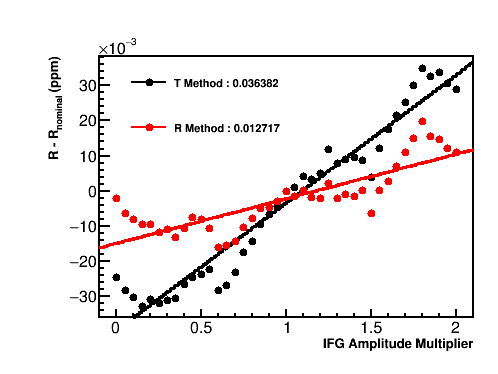
\includegraphics[width=\textwidth]{IFG_Amplitude_Compare_R}
        % \caption{}
    \end{subfigure}% %you need this % here to add spacing between subfigures
    \hspace{1cm}
    \begin{subfigure}[t]{0.45\textwidth}
        \centering
        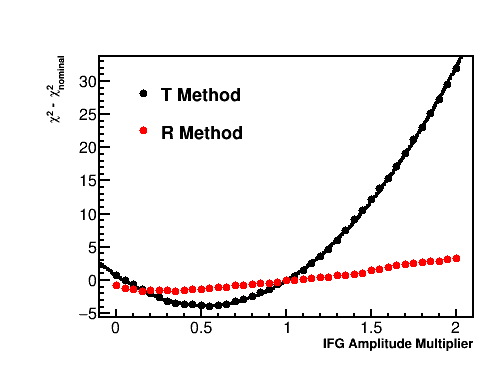
\includegraphics[width=\textwidth]{IFG_Amplitude_Compare_Chisq}
        % \caption{}
    \end{subfigure}
\caption[]{\R (left) and \chisq (right) versus the multiplier on the IFG amplitude parameter, for the T- and R-Methods. The sensitivities of \R to the parameter is determined by fitting a line to the points in the range 0--2, and the extracted values are included in the plot in units of ppm per unit amplitude. It should be noted that the fluctuations in the points are statistical in nature. As shown the sensitivity of the R-Method to the IFG amplitude is less than that of the T-Method. For the \chisq plot, the T-Method forms a parabola and finds a minimum far from the nominal multiplier of 1, which is evidence for the need for a residual gain correction; see \secref{sub:residual_gain_correction}. The R-Method with it's reduced sensitivity does not form a parabola. Data are from the 60h dataset.}
\label{fig:IFGAmpscan}
\end{figure}



\begin{figure}[h]
\centering
    \begin{subfigure}[t]{0.45\textwidth}
        \centering
        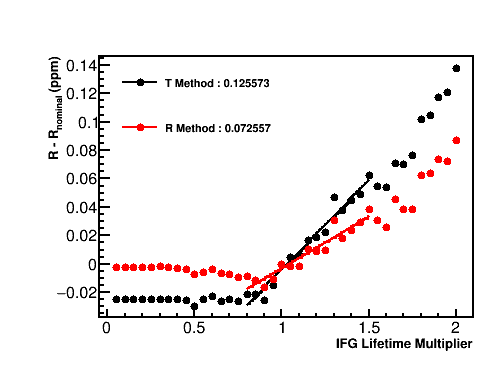
\includegraphics[width=\textwidth]{IFG_Lifetime_Compare_R}
        % \caption{}
    \end{subfigure}% %you need this % here to add spacing between subfigures
    \hspace{1cm}
    \begin{subfigure}[t]{0.45\textwidth}
        \centering
        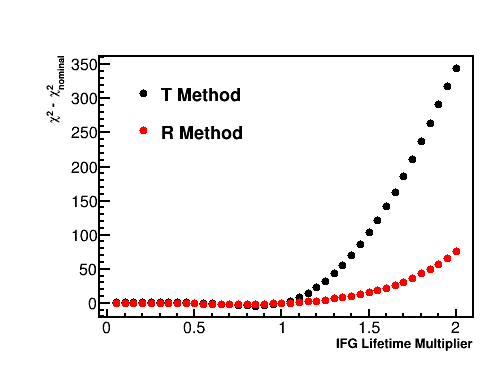
\includegraphics[width=\textwidth]{IFG_Lifetime_Compare_Chisq}
        % \caption{}
    \end{subfigure}
\caption[]{\R (left) and \chisq (right) versus the multiplier on the IFG time constant parameter, for the T- and R-Methods, for the 60h dataset. The sensitivities of \R to the parameter is determined by fitting a line to the points in the range 0.8--1.5, and the extracted values are included in the plot in units of ppm per unit time constant. As shown the sensitivity of the R-Method to the IFG amplitude is less than that of the T-Method.}
\label{fig:IFGtauscan}
\end{figure}


\begin{figure}[h]
\centering
    \begin{subfigure}[t]{0.45\textwidth}
        \centering
        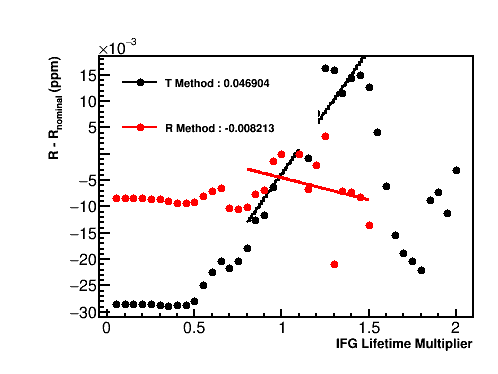
\includegraphics[width=\textwidth]{IFG_Lifetime_Compare_R_9d}
        % \caption{}
    \end{subfigure}% %you need this % here to add spacing between subfigures
    \hspace{1cm}
    \begin{subfigure}[t]{0.45\textwidth}
        \centering
        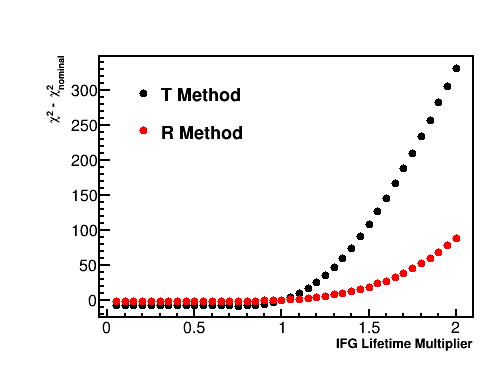
\includegraphics[width=\textwidth]{IFG_Lifetime_Compare_Chisq_9d}
        % \caption{}
    \end{subfigure}
\caption[]{\R (left) and \chisq (right) versus the multiplier on the IFG time constant parameter, for the T- and R-Methods, for the 9d dataset. The sensitivities of \R to the parameter is determined by fitting a line to the points in the range 0.8--1.5, and the extracted values are included in the plot in units of ppm per unit time constant. As shown the sensitivity of the R-Method to the IFG amplitude is less than that of the T-Method. \R versus the time constant for the 9d and Endgame datasets falls off at high multipliers, due to a different procedure for determining the time constants in the IFG correction in those two datasets.}
\label{fig:IFGtauscan9d}
\end{figure}





\tabref{tab:IFGResults} gives the sensitivities to the IFG amplitude and time constant parameters for the four Run~1 datasets, and the associated systematic errors after those sensitivities have been multiplied against the corresponding errors in \tabref{tab:gainCorrErrs}. As shown the errors are small, $\mathcal{O}(10)$ ppb. 




\begin{table}[h]
\centering
% \setlength\tabcolsep{10pt}
\renewcommand{\arraystretch}{1.2}
\begin{tabularx}{0.9\linewidth}{XcYKYK}
  \hline
    \multicolumn{6}{c}{\textbf{IFG Systematic Uncertainties}} \\
  \hline\hline
    Dataset & \thead{Fit Method} & \multicolumn{1}{c}{$dR/dA_{IFG}$} & \multicolumn{1}{c}{$\boldsymbol{\delta R_{A_{IFG}}}$} & \multicolumn{1}{c}{$dR/d\tau_{IFG}$} & \multicolumn{1}{c}{$\boldsymbol{\delta R_{\tau_{IFG}}}$} \\
  \hline
    \multirow{2}{*}{60h} & T & 36.4 & 7.8 & 125.6 & 20.2 \\
                         & R & 12.7 & 2.7 & 72.6 & 11.7 \\
  \hline
    \multirow{2}{*}{HighKick} & T & 52.1 & 3.3 & 150.4 & 9.8 \\
                              & R & 8.4 & 0.5 & 49.7 & 3.2 \\
  \hline
    \multirow{2}{*}{9d} & T & 29.6 & 4.5 & 46.9 & 5.4 \\
                        & R & 9.7 & 1.5 & 8.2 & 0.9 \\
  \hline
    \multirow{2}{*}{Endgame} & T & 64.0 & 2.4 & 204.5 & 13.3 \\
                             & R & 27.9 & 1.0 & 101.3 & 6.6 \\
  \hline
\end{tabularx}
\caption[]{Sensitivities of \R to IFG parameters for the four Run~1 datasets and associated systematic errors in bold. Units are in ppb per unit amplitude, ppb per unit time constant, and ppb, for the sensitivities and systematic uncertainties respectively.}
\label{tab:IFGResults}
\end{table}





\clearpage
\subsection{STDP}


The systematic uncertainty due to the STDP correction was evaluated by turning the STDP correction entirely off before reclustering the hits and refitting the data. The change in \R, \DR, was multiplied by the uncertainty in the STDP amplitude as given in \tabref{tab:gainCorrErrs} to determine the systematic uncertainty. The Run~1 analysis did not have the capability to scan over the STDP parameters as was done for the IFG, hence the single point chosen with an amplitude of 0\footnote{This has been fixed for future analyses.}. It should be noted that because of the nature of how the randomization is applied in the BU analysis, the change in \R was completely disassociated from any randomization effects, and is solely due to the change in gain. \tabref{tab:systematicError_STDP} gives the \DR's with the STDP turned off, along with the systematic uncertainties for the four datasets and both fit methods. As shown the systematic uncertainties are entirely negligible at less than 1~ppb. Because the systematic uncertainties were so small, a systematic uncertainty regarding the STDP time constant was not evaluated.


\begin{table}[h]
\centering
% \setlength\tabcolsep{10pt}
\renewcommand{\arraystretch}{1.2}
\begin{tabularx}{0.7\linewidth}{XOOK}
  \hline
    \multicolumn{4}{c}{\textbf{STDP Systematic Uncertainties}} \\
  \hline\hline
    Dataset & \thead{Fit Method} & \multicolumn{1}{c}{$\Delta R_{\text{(w/ - w/o)}}$} & \multicolumn{1}{c}{$\boldsymbol{\delta R}$} \\
  \hline
    \multirow{2}{*}{60h} & T & 4.8 & 0.1 \\
                         & R & 2.8 & 0.1 \\
  \hline
    \multirow{2}{*}{HighKick} & T & 2.2 & 0.1 \\
                              & R & 2.2 & 0.1 \\
  \hline
    \multirow{2}{*}{9d} & T & 11.2 & 0.2 \\
                        & R & 14.0 & 0.3 \\
  \hline
    \multirow{2}{*}{Endgame} & T & 3.9 & 0.1 \\
                             & R & 5.0 & 0.1 \\
  \hline
\end{tabularx}
\caption[]{Changes in \R with versus without the STDP effect applied for both fit methods for all four datasets, along with the associated systematic uncertainties. These uncertainties were evalued by multiplying the \DR's by the error on the STDP amplitude parameters as given in \tabref{tab:gainCorrErrs}. Units are in ppb.}
\label{tab:systematicError_STDP}
\end{table}








\subsection{Residual Gain Correction}
\label{sub:residual_gain_correction}


In Run~1 (and potentially for future runs) there were several pieces of evidence that pointed towards the need for a residual or ad-hoc gain correction \footnote{It might not actually be a gain effect, and may instead be something like an acceptance effect, however that is the terminology that has been used so the author is sticking with it here.}. These included fit start time scans for the $N$, $\tau_{\mu}$, and \K parameters which fell outside the $1\sigma$ allowed difference bands, IFG amplitude scans which found minima far from the nominal multiplier of 1 (see \figref{fig:IFGAmpscan}), and the \K versus energy spectra which falls at high energies as opposed to remaining constant \cite{phdthesis:2020Sweigart,phdthesis:2019Fienberg,AdHoc1,AdHoc2}. A. Fienberg proposed an additional gain correction with the form
\begin{align}
  E_{c} = E_{m} \cdot (1 + A_{g} e^{-t/\tau_{\mu}} (1 + 0.2 \cos(\omega_{a}t + \phi))),
\end{align}
where $E_{c}$ is the corrected energy of the detected positron, $E_{m}$ is it's measured energy, and $A_{g}$ is the amplitude of the correction. The asymmetry value of 0.2 on the oscillatory part was determined as the ``overall asymmetry of the energy-weighted hit rate'' \cite{phdthesis:2019Fienberg}. \taumu was set to the nominal time-dilated muon lifetime of \SI{64440}{}~ns, while \wa and $\phi$ were set to those values determined from fits to the different datasets without the residual gain correction.


By applying this residual gain correction to the cluster energies with the right amplitude, each of the aforementioned issues disappears. Two procedures were utilized to determine what the value of the amplitude should be. The first was by doing a scan over the residual gain amplitude, as in the IFG amplitude, and finding the minimum, as shown in \figref{fig:AdHocGainScan}\footnote{Scans over the asymmetry value were also performed, and minima were found which agreed with the nominal value of 0.2.}. The second, more physically motivated procedure, was to determine the amplitude as that which flattened out the \K versus energy spectrum. This was done by performing energy bin fits using the T-Method, including just the main CBO parameters in the fit, as shown in \figref{fig:EBinKloss}. Depending on dataset, the amplitudes for both these procedures had values of 0.5--1$\times 10^{-3}$. The \chisq procedure produced an equal amplitude to that of the flag \K procedure for the 60h dataset, higher amplitudes for the HighKick and 9d datasets, and a smaller amplitude for the Endgame dataset. \tabref{tab:AdHocGainTests} compares directly the the different amplitudes between the two procedures, and the associated p-values as determined from straight line fits in the range \SIrange{1.1}{3.1}{\GeV} after applying the residual gain correction with the associated amplitudes. 



\begin{figure}[h]
\centering
    \begin{subfigure}[t]{0.45\textwidth}
        \centering
        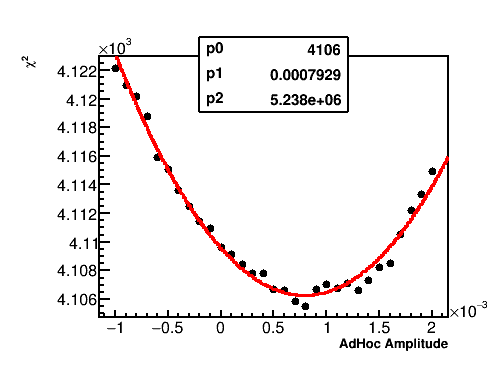
\includegraphics[width=\textwidth]{TMethod_Chi2_Vs_AdHocAmplitude_Canv}
        \caption{T-Method \chisq versus residual gain amplitude. The parabolic fit equation used was $y = p_{2}(x - p_{1})^{2} + p_{0}.$}
    \end{subfigure}% %you need this % here to add spacing between subfigures
    \hspace{1cm}
    \begin{subfigure}[t]{0.45\textwidth}
        \centering
        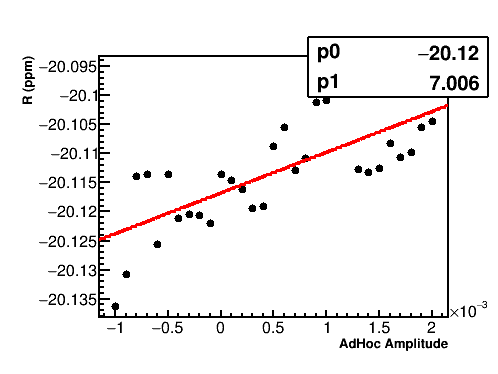
\includegraphics[width=\textwidth]{TMethod_R_Vs_AdHocAmplitude_Canv}
        \caption{T-Method $R$ versus residual gain amplitude. The parameter $p_{1}$ gives the sensitivity of $R$ to the value of the residual gain amplitude, with units in ppm per unit amplitude.}
    \end{subfigure}

    \begin{subfigure}[t]{0.45\textwidth}
        \centering
        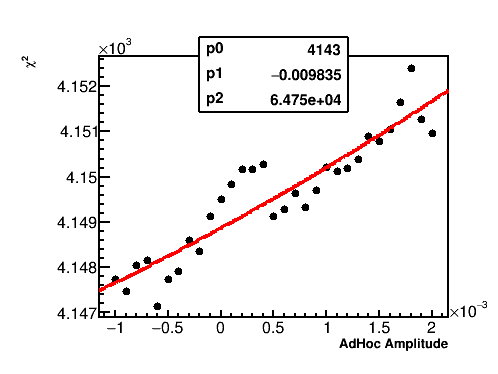
\includegraphics[width=\textwidth]{FullRatio_Chi2_Vs_AdHocAmplitude_Canv}
        \caption{R-Method \chisq versus residual gain amplitude. The parabolic fit equation used was $y = p_{2}(x - p_{1})^{2} + p_{0}.$}
    \end{subfigure}% %you need this % here to add spacing between subfigures
    \hspace{1cm}
    \begin{subfigure}[t]{0.45\textwidth}
        \centering
        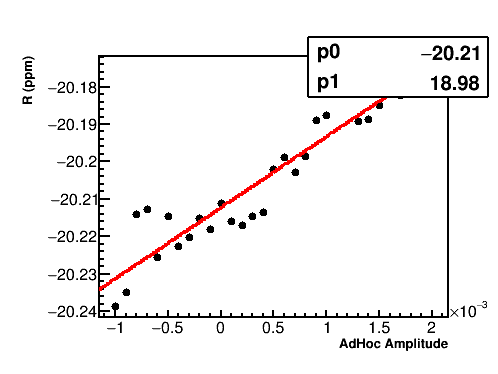
\includegraphics[width=\textwidth]{FullRatio_R_Vs_AdHocAmplitude_Canv}
        \caption{R-Method $R$ versus pileup multiplier. The parameter $p_{1}$ gives the sensitivity of $R$ to the value of the pileup multiplier, with units in ppm per unit amplitude.}
    \end{subfigure}
\caption[]{Residual gain amplitude scan. The \chisq for the R-Method is less sensitive to the residual gain correction than that for the T-Method, hence the lack of a clear parabolic shape. However, the sensitivity of the two methods is comparable, oweing to the fact that the \wa component in the residual gain correction affects both datasets more or less equally. Data are from the 60h dataset.}
\label{fig:AdHocGainScan}
\end{figure}



\begin{landscape}
\begin{figure}[h]
\centering
    \begin{subfigure}[t]{0.34\textwidth}
        \centering
        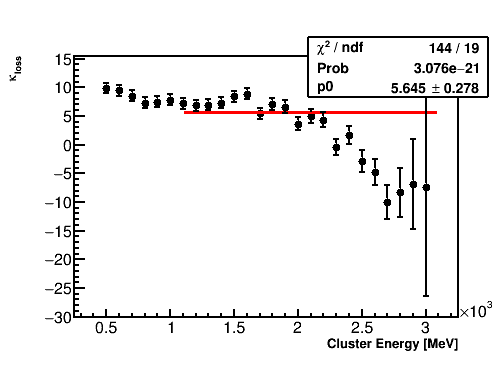
\includegraphics[width=\textwidth]{TMethod_kappa_loss_Vs_EBin_Canv_HK-0}
        \caption{HighKick dataset, $A_{g} = 0$, no residual gain applied.}
    \end{subfigure}% %you need this % here to add spacing between subfigures
    \hspace{1cm}
    \begin{subfigure}[t]{0.34\textwidth}
        \centering
        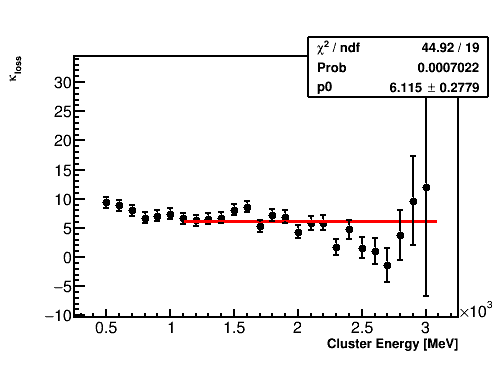
\includegraphics[width=\textwidth]{TMethod_kappa_loss_Vs_EBin_Canv_HK-5p1}
        \caption{HighKick dataset, $A_{g} = 5.1 \times 10^{-4}$, amplitude set to that from the \chisq minima.}
    \end{subfigure}
    \hspace{1cm}
    \begin{subfigure}[t]{0.34\textwidth}
        \centering
        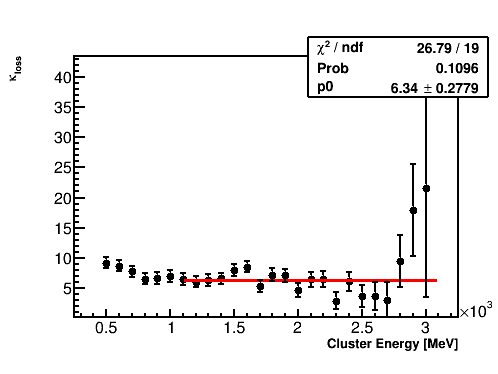
\includegraphics[width=\textwidth]{TMethod_kappa_loss_Vs_EBin_Canv_HK-7p5}
        \caption{HighKick dataset, $A_{g} = 7.5 \times 10^{-4}$, amplitude set to that which flattened out the \K spectrum (approximately).}
    \end{subfigure}

    \begin{subfigure}[t]{0.34\textwidth}
        \centering
        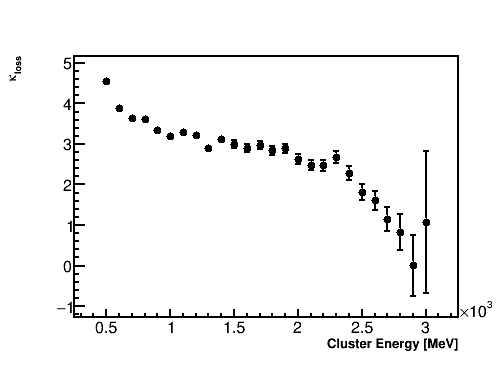
\includegraphics[width=\textwidth]{TMethod_kappa_loss_Vs_EBin_Canv_EG-0}
        \caption{Endgame dataset, $A_{g} = 0$, no residual gain applied.}
    \end{subfigure}% %you need this % here to add spacing between subfigures
    \hspace{1cm}
    \begin{subfigure}[t]{0.34\textwidth}
        \centering
        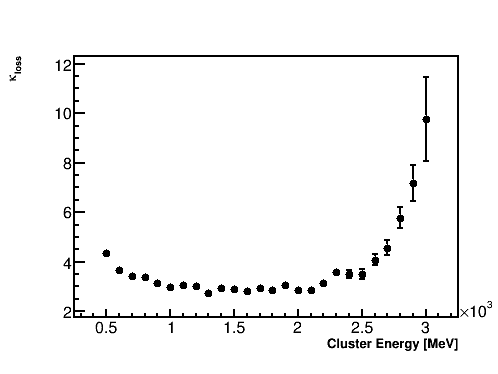
\includegraphics[width=\textwidth]{TMethod_kappa_loss_Vs_EBin_Canv_EG-11p2}
        \caption{Endgame dataset, $A_{g} = 11.2 \times 10^{-4}$, amplitude set to that from the \chisq minima.}
    \end{subfigure}
    \hspace{1cm}
    \begin{subfigure}[t]{0.34\textwidth}
        \centering
        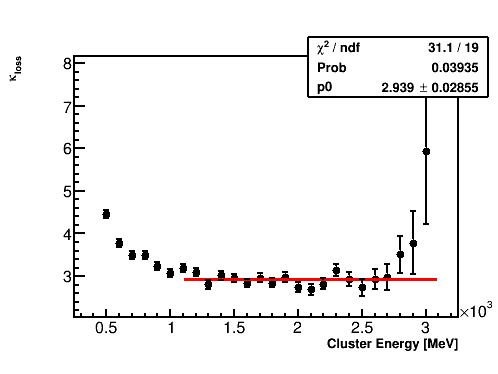
\includegraphics[width=\textwidth]{TMethod_kappa_loss_Vs_EBin_Canv_EG-6p0}
        \caption{Endgame dataset, $A_{g} = 6.0 \times 10^{-4}$, amplitude set to that which flattened out the \K spectrum (approximately).}
    \end{subfigure}
\caption[]{\K versus energy bin, for the HighKick (top) and Endgame (bottom) datasets, with different values for the residual gain amplitude $A_{g}$. \K falls off as a function of energy which is one of the pieces of evidence for the need for a residual gain correction. At low energies \K rises, which is understood to be due to noise hits which increases the lost muon counts at those energies.}
\label{fig:EBinKloss}
\end{figure}
\end{landscape}



\begin{table}[h]
\centering
% \setlength\tabcolsep{10pt}
\renewcommand{\arraystretch}{1.2}
\begin{tabularx}{0.7\linewidth}{XHGHG}
  \hline
    \multicolumn{5}{c}{\textbf{Residual Gain Tests}} \\
  \hline\hline
            & \multicolumn{2}{c}{$\chi^{2}_{min}$} & \multicolumn{2}{c}{flat $\kappa_{loss}$} \\
  \cmidrule(lr){2-3}\cmidrule(lr){4-5}
    Dataset & \multicolumn{1}{c}{$A_{g} \times 10^{-4}$} & \multicolumn{1}{c}{p value} & \multicolumn{1}{c}{$A_{g} \times 10^{-4}$} & \multicolumn{1}{c}{p value} \\
  \hline
    60h & 8.5 & 0.81 & 8.5 & 0.81 \\
    HighKick & 5.1 & \sim 0 & 7.5 & 0.11 \\
    9d & 8.4 & 0.17 & 10.0 & 0.25 \\
    Endgame & 11.2 & \sim 0 & 6.0 & 0.04 \\
  \hline
\end{tabularx}
\caption[]{Residual gain amplitudes as determined from the \chisq minima or flat \K procedures. p-values are given for a straight fit line to the \K versus energy bin spectra from \SIrange{1.1}{3.1}{\GeV} after applying the residual gain correction with the respective amplitudes in the table.}
\label{tab:AdHocGainTests}
\end{table}



\tabref{tab:AdHocGainErr} gives the \DR values when applying the residual gain correction to the four datasets for the two fit methods. These \DR values with minus without the correction are taken conservatively as the systematic uncertainty due to the potential need for such a residual gain correction. Because the flat \K procedure is more physically motivated, the associated values are taken as the final systematic uncertainties. As shown the systematic uncertainties range up to about 30~ppb depending on the dataset, and is one of the larger systematic uncertainties in the analysis.


As a last note, it should immediately be apparent that the \K energy spectrum was not perfectly flat, even with the residual gain correction applied. Beyond random statistical fluctuations, it rises up at high energy bins, and no $A_{g}$ value was found which could better flatten out the spectrum. This is understood to be an effect of the pileup correction applied, potentially due to the lack of triples included in the correction. With a better pileup algorithm, this effect should go away. Because the systematic uncertainty is taken conservatively as the \DR value with minus without the correction applied, and because the magnitude of the uncertainties was comparable to analyses without this defect, this was deemed acceptable for the Run~1 analysis.




\begin{table}[h]
\centering
% \setlength\tabcolsep{10pt}
\renewcommand{\arraystretch}{1.2}
\begin{tabularx}{0.8\linewidth}{XOOK}
  \hline
    \multicolumn{4}{c}{\textbf{Systematic Uncertainty Due to Residual Gain}} \\
  \hline\hline
    Dataset & \thead{Fit Method} & \multicolumn{1}{c}{$\chi^{2}_{min}$ $\Delta R$} & \multicolumn{1}{c}{flat $\kappa_{loss}$ $\boldsymbol{\Delta R}$}  \\
  \hline
    \multirow{2}{*}{60h} & T & 28.7 & 28.7 \\
                         & R & 22.9 & 22.9 \\
  \hline
    \multirow{2}{*}{HighKick} & T & 1.0 & 11.8 \\
                              & R & 1.8 & 15.3 \\
  \hline
    \multirow{2}{*}{9d} & T & 18.1 & 24.4 \\
                        & R & 15.2 & 19.1 \\
  \hline
    \multirow{2}{*}{Endgame} & T & 29.9 & 18.8 \\
                             & R & 8.5 & 6.7 \\
  \hline
\end{tabularx}
\caption[]{Systematic uncertainties due to the potential need for a residual gain correction, with an applied amplitude determined from either the minimum of a \chisq scan or that which flattened out the \K versus energy spectra. The latter column is bold reflecting the fact that those numbers were the final reported systematic uncertainties. In general both procedures produce the same order of magnitude systematic uncertainties, except for the HighKick where the latter procedure produces larger values. Units are in ppb.}
\label{tab:AdHocGainErr}
\end{table}




%!TEX root = ../BUSystematics.tex

\graphicspath{{Body/Figures/Pileup/}{Body/Figures/Pileup/Amplitude/}{Body/Figures/Pileup/TimeShift/}{Body/Figures/Pileup/EnergyModel/}{Body/Figures/Pileup/TriplePileup/}{Body/Figures/Pileup/RateError/}}

\section{Pileup}

The pileup correction used in the BU analysis is the asymmetric shadow window method. Extensive details can be found in \refref{phdthesis:2020Kinnaird}; here is given a brief summary. A pileup correction is constructed by looking in ``shadow'' time windows some time after ``trigger'' pulses for trailing shadow pulses. The assumption is that the probability for a pileup event to occur is the same as that to find a shadow pulse trailing a trigger pulse in the right length time window. By looking in all such shadow windows for all trigger pulses and constructing ``shadow doublets,'' a pileup correction is constructed and then applied to the data. The length of the shadow window is called the ``shadow dead time,'' and the gap time between the trigger pulse time and the start of the shadow window is called the ``shadow gap time.''  \tabref{tab:pileupParameters} gives the parameter values for the pileup parameters. The shadow gap time of \ns{10} was chosen to be suitably small such that the event rate was marginally different from the real pileup rate at the trigger pulse time. The shadow dead time of \ns{4.06} was determined by scanning over shadow dead times and finding the value at which the ratio of pileup energies over measured energies in the range \SIrange{3.5}{4.5}{\GeV} was equal to 1, where pileup doublets make up almost the entirety of the counts\footnote{This value of \ns{4.06} is a direct effect of the clustering dead time of 3~cts applied to the Run~1 datasets for ReconWest. With this shadow dead time applied in the procedure, no additional nominal multiplier beyond 1 is applied to the pileup amplitude as was done in the author's dissertation, or other shadow methods.}. On a separate but important note, in the final analysis no local artificial dead time was applied to the incoming clusters. This is in comparison to the analysis done for the dissertation in which an artificial dead time of \ns{5} was applied to the incoming clusters \cite{phdthesis:2020Kinnaird}.


\begin{table}[h]
\centering
% \setlength\tabcolsep{10pt}
\renewcommand{\arraystretch}{1.2}
\begin{tabularx}{0.4\linewidth}{lc}
  \hline
    \multicolumn{2}{c}{\textbf{Pileup Parameters}} \\
  \hline\hline
    Parameter & \thead{Value} \\
  \hline
    Shadow dead time & 4.06~ns \\
    Shadow gap time $(T_{G})$ & 10~ns \\ 
    Pileup energy scaling $(C)$ & 1 \\
  \hline
\end{tabularx}
\caption[]{}
\label{tab:pileupParameters}
\end{table}


The time and energy models for the shadow pileup construction are given as
        \begin{gather}
            E_{\text{doublet}} = C \cdot (E_{\rm T} + E_{\rm S}), \label{eq:Edoublet} \\
            t_{\text{doublet}} = \frac{t_{\rm T} \cdot E_{\rm T} + (t_{\rm S}-T_{G}) \cdot E_{\rm S}}{E_{\rm T} + E_{\rm S}} + \frac{T_{G}}{2}, \label{eq:tdoublet}
        \end{gather}
where $E_{\text{doublet}}$ and $t_{\text{doublet}}$ are the energies and times of the constructed shadow doublets, and $E_{T}$, $E_{S}$, $t_{T}$, $t_{S}$, are the energies and times of the trigger and shadow pulses respectively. $C$ is an energy scaling parameter with a nominal value of 1, and $T_{G}$ is the shadow gap time. The energy of the constructed shadow doublet is simply the sum of the two singlets, while the time is the energy weighted time of the two singlets plus a time-shift of $\frac{T_{G}}{2}$. This time-shift accounts for the fact that combining two pulses with a shift of $T_{G}$ between them is most representative (approximately) of the pileup rate with a time-shift of $T_{G}/2$ on the constructed shadow doublet.


Systematic uncertainties arise primarily from uncertainties in the pileup correction amplitude, as well as the time and energy models used. Others include uncertainties due to the pileup rate, unseen pileup, and the omission of triples in the correction. No systematic uncertainty was evaluated in regards to an artificial dead time since none was applied in the analysis beyond that in the clustering.



\subsection{Amplitude}

The pileup amplitude uncertainty was evaluated by applying multipliers to the amplitude of the pileup correction, and refitting the data. Multipliers were applied in steps of 0.01 from 0.9 to 1.1, and the resulting \R vs pileup multiplier plot was fit to determine the sensitivity of \R to the pileup multiplier. The uncertainty in the multiplier was determined as the width of the parabola in the \chisq vs pileup multiplier plot. The systematic uncertainty on \R was then calculated as 
    \begin{align}
        \delta R = \sigma_{P_{m}} \times \frac{dR}{dP_{m}},
    \end{align}
where $P_{m}$ is the value of the pileup multiplier. \figref{fig:PMscan} shows the scan results for the 9d dataset. \tabref{tab:pileupMultplierScan} show the scan results and \tabref{tab:systematicError_pileupMultplier} gives the systematic uncertainties for each of the Run~1 datasets.





\begin{table}[h]
\centering
% \setlength\tabcolsep{10pt}
\renewcommand{\arraystretch}{1.2}
\begin{tabularx}{0.7\linewidth}{XOOOO}
  \hline
    \multicolumn{5}{c}{\textbf{Pileup Amplitude Scan Results}} \\
  \hline\hline
    Dataset & \thead{Fit Method} & \multicolumn{1}{c}{$dR/dP_{m}$} & \multicolumn{1}{c}{$\sigma_{P_{m}}$} & \multicolumn{1}{c}{$P_{m_{\text{min}}}$} \\
  \hline
    \multirow{2}{*}{60h} & T & $-353.1$ & 0.061 & 0.981 \\
                         & R & $-308.3$ & 0.064 & 1.014 \\
  \hline
    \multirow{2}{*}{HighKick} & T & $-235.2$ & 0.049 & 0.981 \\
                              & R & $-217.0$ & 0.053 & 0.982 \\
  \hline
    \multirow{2}{*}{9d} & T & $-187.8$ & 0.043 & 0.988 \\
                        & R & $-217.6$ & 0.046 & 1.002 \\
  \hline
    \multirow{2}{*}{Endgame} & T & $-326.4$ & 0.031 & 0.879 \\
                             & R & $-269.0$ & 0.035 & 0.958 \\
  \hline
\end{tabularx}
\caption[]{Results for pileup amplitude multiplier scans for the four Run~1 datasets for both fit methods. Include are the sensitivities of \R to the pileup multiplier, uncertainty on the amplitude as determined from the width of the \chisq parabolas, and the pileup multiplier for which the \chisq was a minimum. The sensitivities are in units of ppb per unit multiplier (or just ppb), and the rest of the quantities are unit-less.}
\label{tab:pileupMultplierScan}
\end{table}


\begin{table}[h]
\centering
\renewcommand{\arraystretch}{1.2}
\begin{tabularx}{0.6\linewidth}{XYY}
  \hline
    \multicolumn{3}{c}{\textbf{Pileup Amplitude Systematic Uncertainties}} \\
  \hline\hline
    Dataset & \thead{T-Method} & \thead{R-Method} \\
  \hline
    60h & 21.7 & 19.9 \\
    HighKick & 11.4 & 11.4 \\
    9d & 8.1 & 10.1 \\ 
    Endgame & 10.1 & 9.4 \\
  \hline
\end{tabularx}
\caption[]{Systematic uncertainties due to the pileup amplitude. Units are in ppb.}
\label{tab:systematicError_pileupMultplier}
\end{table}


\begin{figure}[h]
\centering
    \begin{subfigure}[t]{0.45\textwidth}
        \centering
        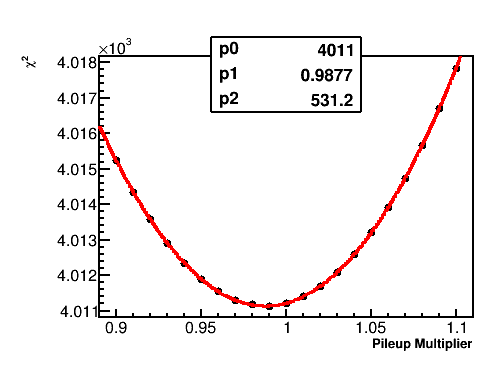
\includegraphics[width=\textwidth]{TMethod_Chi2_Vs_PileupMultiplier_Canv}
        \caption{T-Method \chisq versus pileup multiplier. The parabolic fit equation used was $y = p_{2}(x - p_{1})^{2} + p_{0}.$}
    \end{subfigure}% %you need this % here to add spacing between subfigures
    \hspace{1cm}
    \begin{subfigure}[t]{0.45\textwidth}
        \centering
        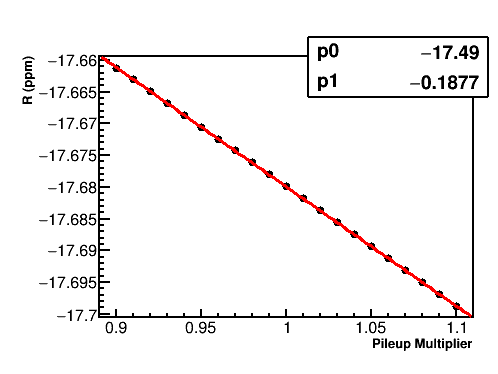
\includegraphics[width=\textwidth]{TMethod_R_Vs_PileupMultiplier_Canv}
        \caption{T-Method $R$ versus pileup multiplier. The parameter $p_{1}$ gives the sensitivity of $R$ to the value of the pileup multiplier, with units in ppm per unit multiplier.}
    \end{subfigure}

    \begin{subfigure}[t]{0.45\textwidth}
        \centering
        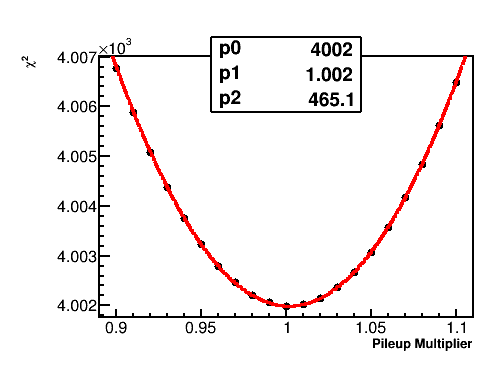
\includegraphics[width=\textwidth]{FullRatio_Chi2_Vs_PileupMultiplier_Canv}
        \caption{R-Method \chisq versus pileup multiplier. The parabolic fit equation used was $y = p_{2}(x - p_{1})^{2} + p_{0}.$}
    \end{subfigure}% %you need this % here to add spacing between subfigures
    \hspace{1cm}
    \begin{subfigure}[t]{0.45\textwidth}
        \centering
        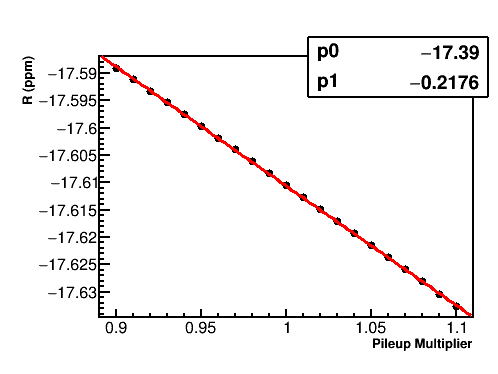
\includegraphics[width=\textwidth]{FullRatio_R_Vs_PileupMultiplier_Canv}
        \caption{R-Method $R$ versus pileup multiplier. The parameter $p_{1}$ gives the sensitivity of $R$ to the value of the pileup multiplier, with units in ppm per unit multiplier.}
    \end{subfigure}
\caption[Pileup multiplier scan]{Pileup multiplier scan. The width of the parabola is determined as the change in X which increases the \chisq by one, which is equal to $1/\sqrt{p_{2}}$. Data are from the 9d dataset.}
\label{fig:PMscan}
\end{figure}



\clearpage
\subsection{Time Model}

The time of a constructed shadow doublet in the pileup construction is set as the energy weighted time of the two singlets plus half the gap time, as shown in \equref{eq:tdoublet}. Previously the uncertainty was calculated by scanning over an additional time-shift parameter and then applying a conservative uncertainty of \ns{2.5} \cite{phdthesis:2020Kinnaird}. The results of such a scan can be seen in \figref{fig:PTSscan}. If this procedure is used then the systematic uncertainty on \R is less than 15~ppb for all datasets. If the most energetic singlet time is set as the doublet time instead, then the $\Delta R$ is less than \ppb{1} for all datasets. Lastly, if the doublet time is set as either the first singlet time, or the second singlet time, then the $\Delta R$'s range approximately from 5--6~ppb, as shown in \tabref{tab:systematicError_clusterTime}. This last approach bounds the possibilities for properly constructed doublet times, and is less conservative than the first approach described, therefore the systematic uncertainty is taken as the average of the absolute values of the two \DR values when using the first and last singlet times. The final systematic uncertainties are also given in \tabref{tab:systematicError_clusterTime} in bold.




\begin{figure}[h]
\centering
    \begin{subfigure}[t]{0.45\textwidth}
        \centering
        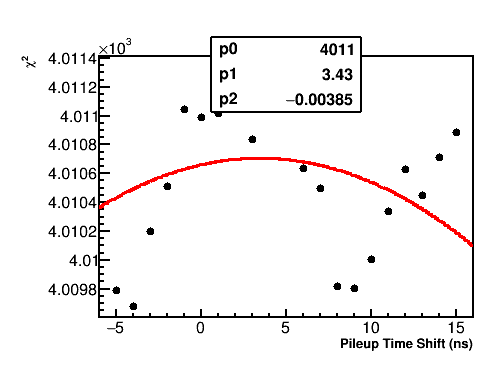
\includegraphics[width=\textwidth]{TMethod_Chi2_Vs_PileupTimeShift_Canv}
        \caption{T-Method \chisq versus pileup time shift. There is no clear parabolic shape or minimum.}
    \end{subfigure}% %you need this % here to add spacing between subfigures
    \hspace{1cm}
    \begin{subfigure}[t]{0.45\textwidth}
        \centering
        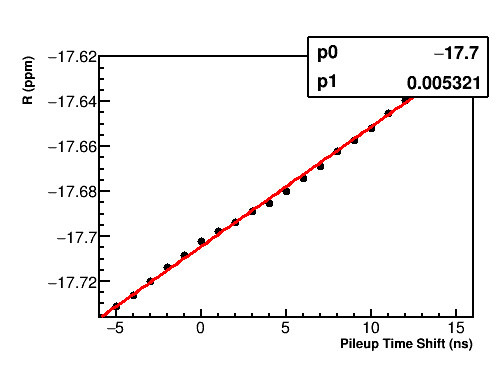
\includegraphics[width=\textwidth]{TMethod_R_Vs_PileupTimeShift_Canv}
        \caption{T-Method $R$ versus pileup time shift. The parameter $p_{1}$ gives the sensitivity of $R$ to the value of the pileup time shift, with units in ppm per ns.}
    \end{subfigure}
\caption[Pileup time shift scan]{Pileup time shift scan for the T-Method. The R-Method plots look the same. There is a wave in the \R plot, but the effect is small and therefore ignored. Data are from the 9d dataset.}
\label{fig:PTSscan}
\end{figure}


\begin{table}[h]
\centering
\renewcommand{\arraystretch}{1.2}
\begin{tabularx}{0.9\linewidth}{@{\extracolsep{\fill}}XHHPHHP}
  \hline
    \multicolumn{7}{c}{Time Model Systematic Uncertainty} \\
  \hline\hline
            & \multicolumn{3}{c}{T-Method} & \multicolumn{3}{c}{R-Method } \\
            \cmidrule(lr){2-4}\cmidrule(lr){5-7}
    Dataset & \thead{First Time} & \thead{Last Time} & \thead{\dR} & \thead{First Time} & \thead{Last Time} & \thead{\dR} \\
  \hline
    60h & -5.5 & 4.6 & 5.1 & -8.0 & 4.8 & 6.4 \\
    HighKick & -5.0 & 4.3 & 4.6 & -5.6 & 4.0 & 4.8 \\
    9d & -5.4 & 5.6 & 5.5 & -5.8 & 5.4 & 5.6 \\ 
    Endgame & -5.5 & 4.4 & 5.0 & -5.2 & 4.3 & 4.8 \\
  \hline
\end{tabularx}
\caption[]{$\Delta R$s when applying either of the two singlet times as the doublet time in the pileup construction, and associated systematic uncertainties calculated as the average of the absolute value of the two values. Units are in ppb.}
\label{tab:systematicError_clusterTime}
\end{table}



% \begin{table}[h]
% \centering
% \renewcommand{\arraystretch}{1.2}
% \begin{tabularx}{0.9\linewidth}{@{\extracolsep{\fill}}XYYYY}
%   \hline
%     \multicolumn{5}{c}{$\Delta R$ with First and Last Singlet Times} \\
%   \hline\hline
%             & \multicolumn{2}{c}{T-Method} & \multicolumn{2}{c}{R-Method } \\
%             \cmidrule(lr){2-3}\cmidrule(lr){4-5}
%     Dataset & \thead{First Time} & \multicolumn{1}{c}{Last Time} & \thead{First Time} & \thead{Last Time}  \\
%   \hline
%     60h & -5.5 & 4.6 & -8.0 & 4.8 \\
%     HighKick & -5.0 & 4.3 & -5.6 & 4.0 \\
%     9d & -5.4 & 5.6 & -5.8 & 5.4 \\ 
%     Endgame & -4.5 & 4.4 & -5.2 & 4.3 \\
%   \hline
% \end{tabularx}
% \caption[]{$\Delta R$ when applying either of the two singlet times as the doublet time in the pileup construction. Units are in ppb.}
% \label{tab:systematicError_clusterTimeDeltas}
% \end{table}





% \begin{table}[h]
% \centering
% \renewcommand{\arraystretch}{1.2}
% \begin{tabularx}{0.5\linewidth}{@{\extracolsep{\fill}}XYY}
%   \hline
%     \multicolumn{3}{c}{\textbf{Time Model Systematic Uncertainty}} \\
%   \hline\hline
%     Dataset & \thead{T-Method} & \thead{R-Method} \\
%   \hline
%     60h & 5.1 & 6.4 \\
%     HighKick & 4.6 & 4.8 \\
%     9d & 5.5 & 5.6 \\ 
%     Endgame & 5.0 & 4.8 \\
%   \hline
% \end{tabularx}
% \caption[]{Systematic uncertainty due to cluster time model. Units are in ppb.}
% \label{tab:systematicError_clusterTimeModel}
% \end{table}





\clearpage
\subsection{Energy Model}

The energy of the shadow doublet in the pileup construction is calculated nominally as the sum of the two singlets, as shown in \equref{eq:Edoublet}. This is an okay approximation as the reconstruction typically assigns the energy of any pileup pulse as such, especially when the spatial separation is turned off as it is in the ReconWest reconstruction. Previously the systematic uncertainty was determined by scanning over the multiplier $C$ on the energy sum from 0.9 to 1.1, taking the slope as the sensitivity, and then multiplying it by the uncertainty determined as in the pileup amplitude systematic uncertainty evaluation (from the width of the \chisq parabola). An example of such a scan is shown in \figref{fig:PESscan}. It was found that the uncertainties as determined from the \chisq ranged from 3--6.4\% depending on the dataset (going smaller with more statistics), with corresponding systematic uncertainties of 5--20~ppb. While some datasets had clear slopes in \R vs the energy scale multiplier, some did not.



\begin{figure}[h]
\centering
    \begin{subfigure}[t]{0.45\textwidth}
        \centering
        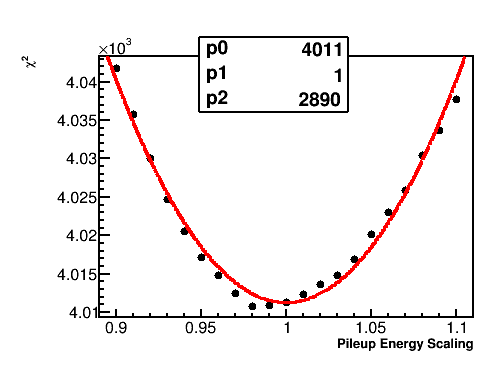
\includegraphics[width=\textwidth]{TMethod_Chi2_Vs_PileupEnergyScaling_Canv}
        \caption{T-Method \chisq versus pileup energy scale. The parabolic fit equation used was $y = p_{2}(x - p_{1})^{2} + p_{0}.$}
    \end{subfigure}% %you need this % here to add spacing between subfigures
    \hspace{1cm}
    \begin{subfigure}[t]{0.45\textwidth}
        \centering
        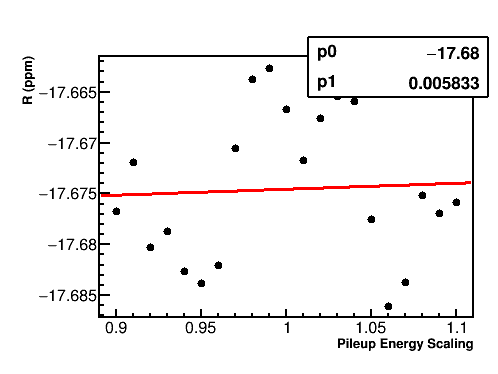
\includegraphics[width=\textwidth]{TMethod_R_Vs_PileupEnergyScaling_Canv}
        \caption{T-Method $R$ versus pileup energy scale. The parameter $p_{1}$ gives the sensitivity of $R$ to the value of the pileup energy scale, with units in ppm per unit scale factor.}
    \end{subfigure}

    \begin{subfigure}[t]{0.45\textwidth}
        \centering
        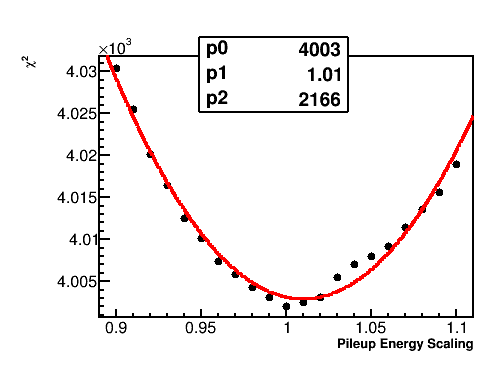
\includegraphics[width=\textwidth]{FullRatio_Chi2_Vs_PileupEnergyScaling_Canv}
        \caption{R-Method \chisq versus pileup energy scale. The parabolic fit equation used was $y = p_{2}(x - p_{1})^{2} + p_{0}.$}
    \end{subfigure}% %you need this % here to add spacing between subfigures
    \hspace{1cm}
    \begin{subfigure}[t]{0.45\textwidth}
        \centering
        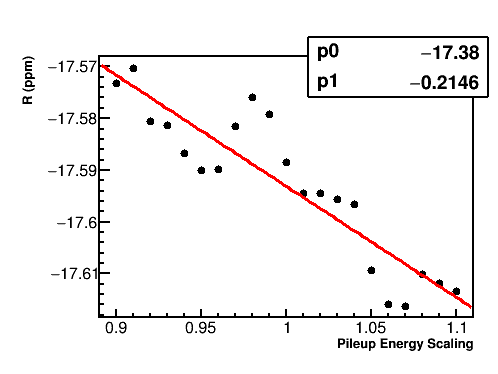
\includegraphics[width=\textwidth]{FullRatio_R_Vs_PileupEnergyScaling_Canv}
        \caption{R-Method $R$ versus pileup energy scale. The parameter $p_{1}$ gives the sensitivity of $R$ to the value of the pileup energy scale, with units in ppm per unit scale factor.}
    \end{subfigure}
\caption[Pileup energy scale scan]{Pileup energy scale scan. Data are from the 9d dataset.}
\label{fig:PESscan}
\end{figure}



Simulations showed however that the energy resolution is much better than that determined by the \chisq; see \figref{fig:ReconEastDoubletEnergyRatios}. Because of this, and because of the non-linear slopes in \R for some datasets, the uncertainty was instead taken as the max $\Delta R$ when applying a $\pm1\%$ scale factor on the doublet energy. This is a reasonable approach, and slightly conservative, as the maximum ratio difference from 1 for energy sums larger than \SI{1.7}{\GeV} is about 1\%. ReconWest is not expected to be significantly different than ReconEast (which was used in the previously mentioned simulations), and the lack of spatial separation would imply that this ratio would be even closer to 1, approximately 0.5\% or so. The systematic uncertainties for the four Run~1 datasets determined via this procedure are given in \tabref{tab:systematicError_clusterEnergyModel}.


\begin{figure}[h]
\centering
    \begin{subfigure}[t]{0.45\textwidth}
        \centering
        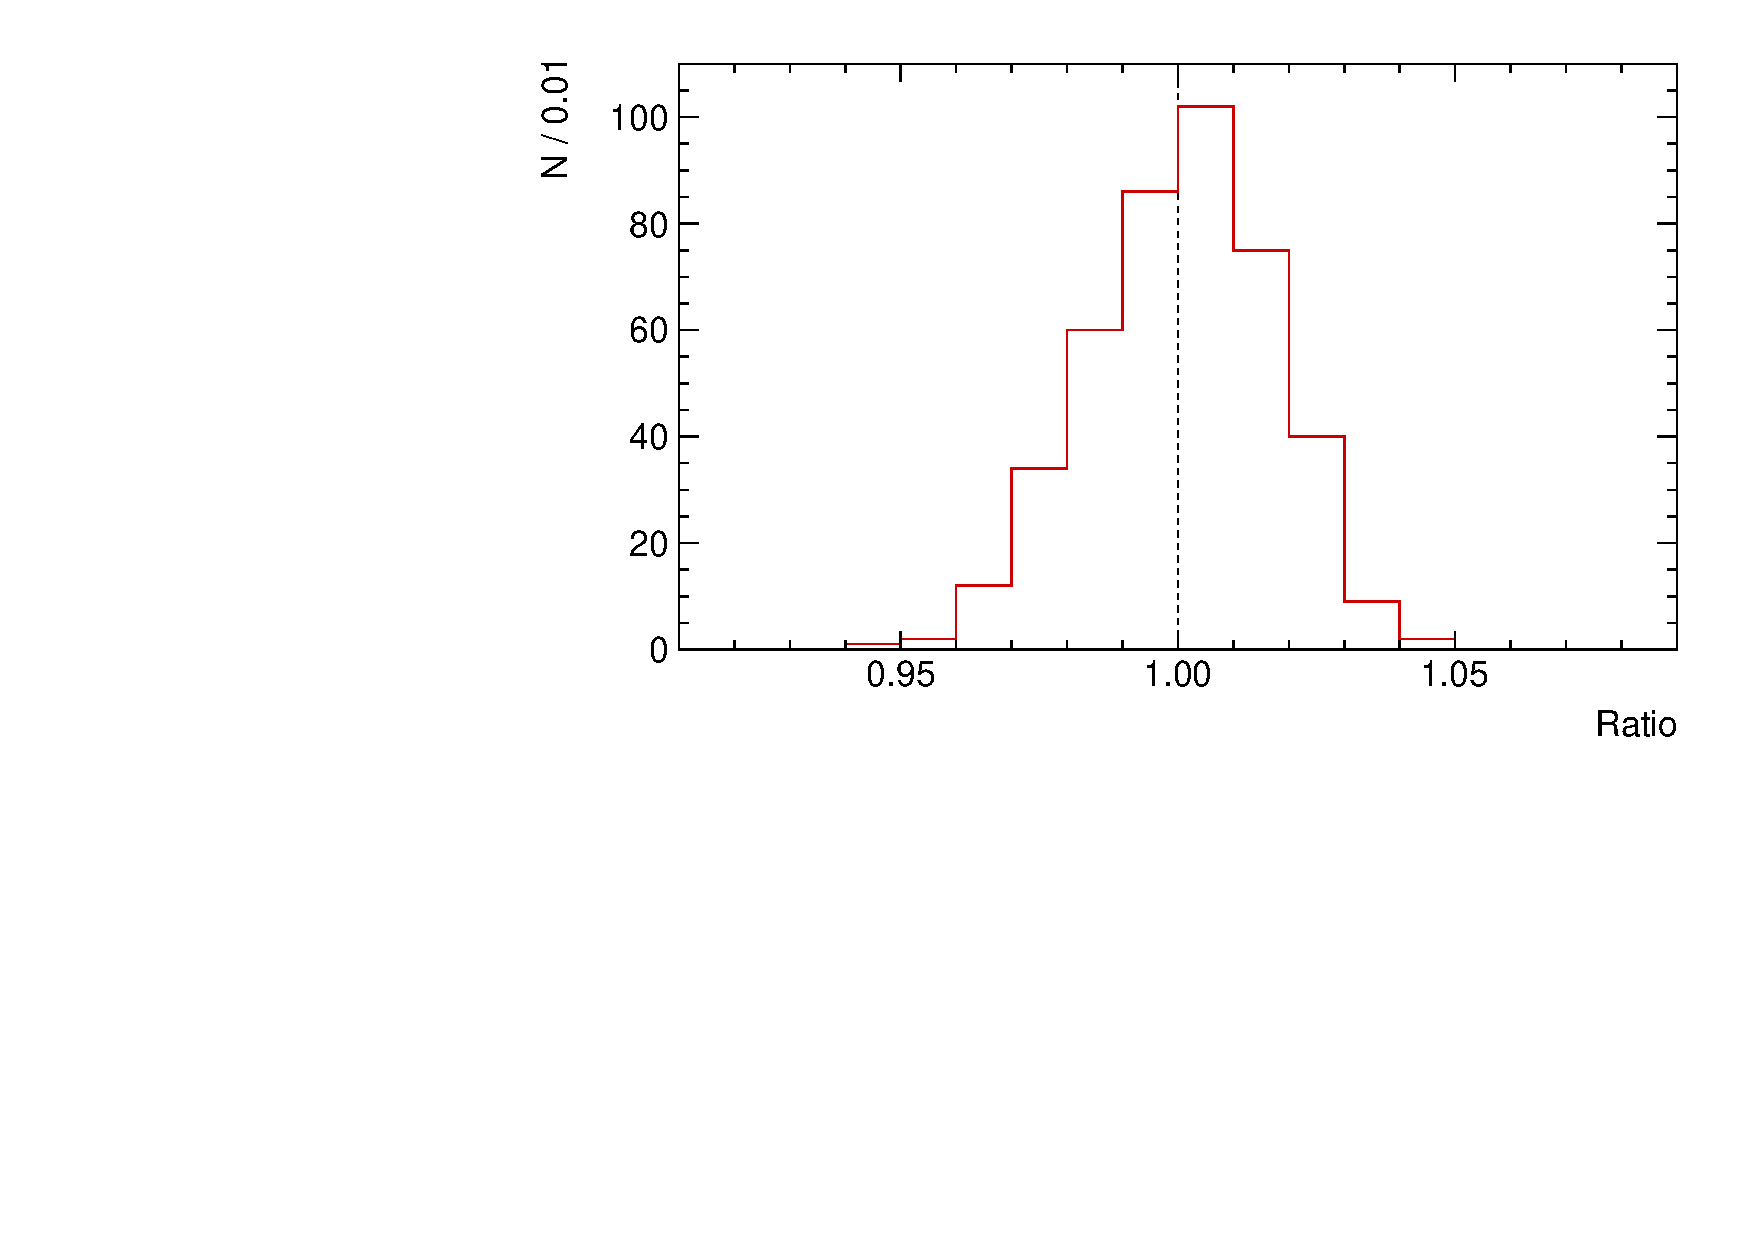
\includegraphics[width=\textwidth]{p_ratio_2_2_hist}
        \caption{The ratio of the doublet energy to the sum of the two singlets for two positrons each with energy 2~\GeV.}
    \end{subfigure}%
    \hspace{1cm}
    \begin{subfigure}[t]{0.45\textwidth}
        \centering
        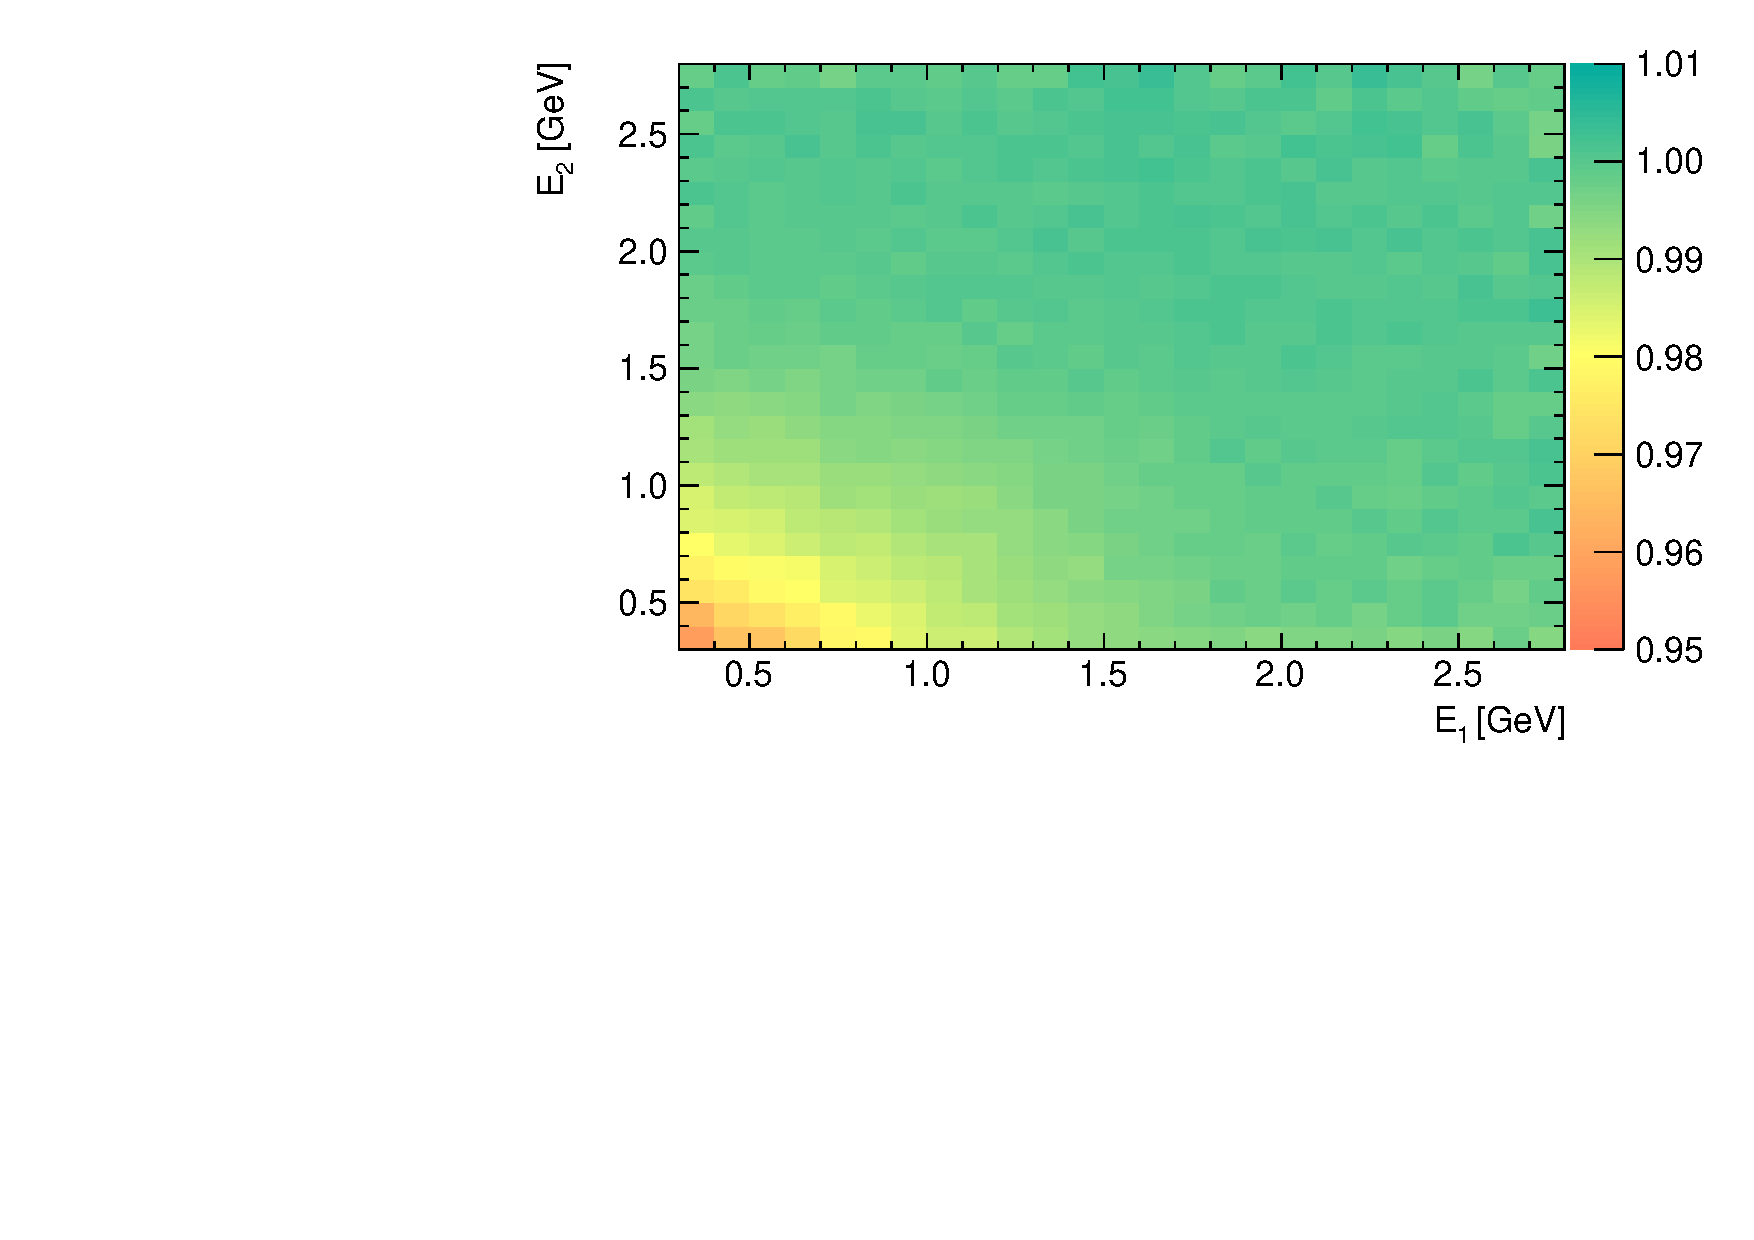
\includegraphics[width=\textwidth]{p_ratio_e1_e2}
        \caption{The average ratio of the doublet energy to the sum of the two singlets as a function of singlet energies.}
    \end{subfigure}
\caption[]{Results from simulations performed by D. Sweigart to determine the ratio of pileup doublet energies to the sum of the two singlets. In the simulations two positrons were fired at the calorimeter using the MDC1 simulation conditions. For cases were pileup occurred, the ratios of the doublet energy to the sum of the two singlets were calculated. The plot on the left is all such energy ratios for the case where the two singlets each had an energy of 2~\GeV, and the plot on the right is the average ratio for all singlet energy combinations. For low energies the ratio can be significantly different from 1, whereas for energies above 1.7~\GeV the difference from 1 is around 1\% or less. Plots courtesy of D. Sweigart.}
\label{fig:ReconEastDoubletEnergyRatios}
\end{figure}


\begin{table}[h]
\centering
\renewcommand{\arraystretch}{1.2}
\begin{tabularx}{0.6\linewidth}{@{\extracolsep{\fill}}XYY}
  \hline
    \multicolumn{3}{c}{\textbf{Energy Model Systematic Uncertainty}} \\
  \hline\hline
    Dataset & \thead{T-Method} & \thead{R-Method} \\
  \hline
    60h & 11.0 & 10.9 \\
    HighKick & 4.8 & 7.2 \\
    9d & 6.1 & 10.2 \\ 
    Endgame & 10.0 & 6.8 \\
  \hline
\end{tabularx}
\caption[]{Systematic uncertainty due to cluster energy model. Units are in ppb.}
\label{tab:systematicError_clusterEnergyModel}
\end{table}




\clearpage
\subsection{Pileup Rate Uncertainty}

A systematic uncertainty from the pileup rate estimation arises from the fact that the pileup is estimated from pulses at times shifted by the gap time $T_{G}$ and then placed with a time-shift $T_{G}/2$. Ideally the pileup would have been estimated at the latter time initially, and there will thus be differences due to muon precession and beam dynamics. Because the gap time used is very small at \ns{10}, this uncertainty can be expected to be negligible. Using the prescription as outlined in D. Sweigart's dissertation \cite{phdthesis:2020Sweigart}, the pileup rate uncertainty was estimated as 
\begin{align}
	\frac{N^{2}(t) - N(t-\frac{T_{G}}{2})N(t+\frac{T_{G}}{2})}{N^{2}(t)},
\end{align}
where $N(t)$ is the fit function determined from a T-Method fit to the data. $N^{2}(t)$ is what should have been used when constructing the pileup, as opposed to $N(t-\frac{T_{G}}{2})N(t+\frac{T_{G}}{2})$. The rate uncertainty is shown in Figures~\ref{fig:pileupRateError} and \ref{fig:pileupRateErrorZoomed}.

There are some interesting features to point out from the figures. The pileup rate uncertainty oscillates at \wa and the shape is constant throughout the fill. The black points in the figure come from the nominal fit, where each graph point is calculated and spaced at 149.2/50~ns = 2.984~ns apart. It turns out that there are spikes at the boundaries of the points as defined in the fit function in ROOT. If instead the fit contains 10x the number of points up to 100,000 as shown in the red graph points, the the spikes accordingly shift, and the shape appears to change. This is an effect of the discretization of the points in the ROOT function used to fit the data. The blue points show the average of the black points over a bin width, and as shown lie in line with the red points. Accounting for the discretization then by averaging over the bin width, the pileup rate uncertainty can be determined from the blue curve and is seen to only wander a maximum of 0.005\%, or 0.00005, away from 0. This is a negligible change in the rate, and the systematic uncertainty is thus taken to be 0 ppb for all datasets. Note that even if the maximum of the black curve were to be taken as the rate uncertainty, then it is still less than 0.04\% or 0.0004 and the systematic uncertainty would still be negligible. As a quick aside, if instead a gap time of \SI{149.2}{\ns} were to be used, the pileup rate uncertainty is significantly larger as shown in \figref{fig:pileupRateErrorLarger}, oscillating between -0.7\% and 0.3\%. This plot is comparable to D. Sweigart's dissertation Figure~6.28. Note that spikes can still be seen in the function due to the discretization, though the relative size of them is much smaller than the rest of the curve.




\begin{figure}
    \centering
    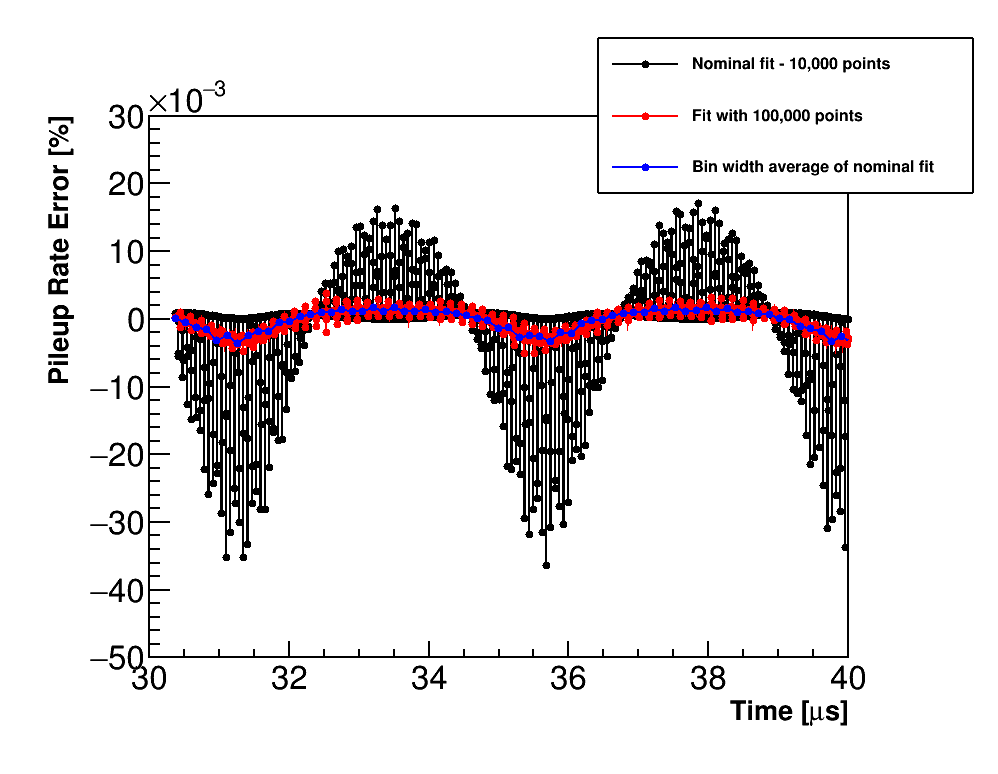
\includegraphics[width=.6\textwidth]{PileupRateError}
    \caption[]{Pileup rate uncertainty with various binning and different numbers of points used in the fit. Black points come from the nominal fit, which includes 10,000 points in the ROOT fit function. Red points come from a fit function with 100,000 points, and the blue points are the average of the black points over bin widths. The scale of the uncertainty or error here is very small, hence the uncertainty on \R is negligible. Data are from the 60h dataset.}
    \label{fig:pileupRateError}
\end{figure}

\begin{figure}
    \centering
    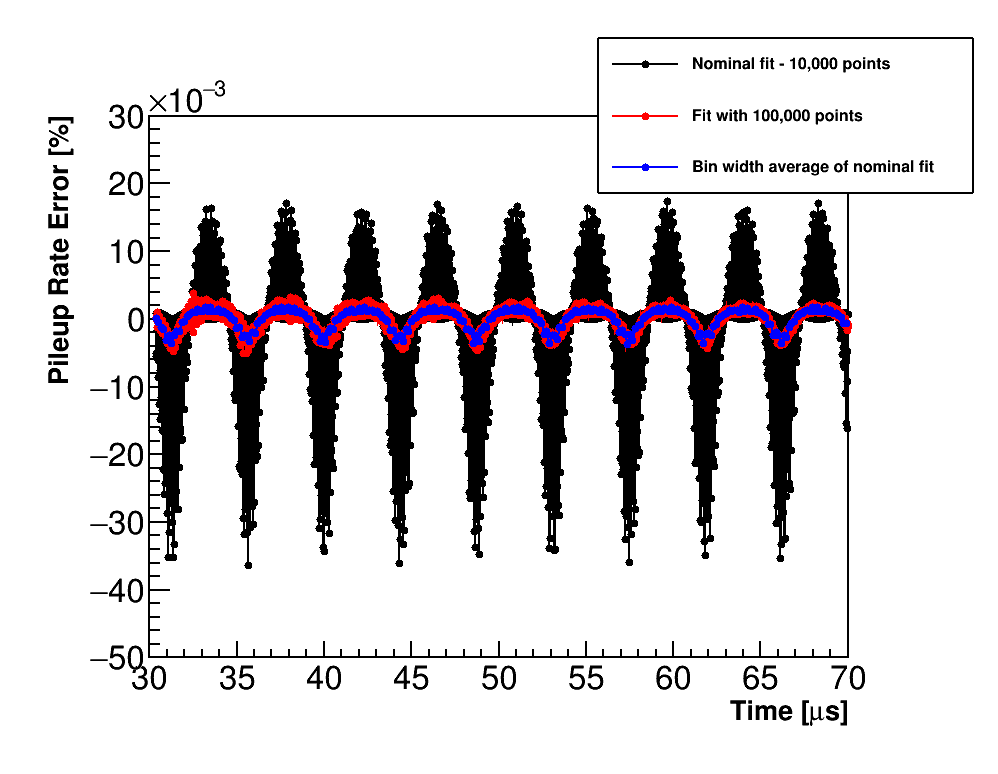
\includegraphics[width=.6\textwidth]{PileupRateError_ZoomedOut}
    \caption[]{Pileup rate uncertainty with various binning and different numbers of points used in the fit. The plot is zoomed out from the previous figure, showing the consistency of the pileup rate uncertainty at later times in the fill. Data are from the 60h dataset.}
    \label{fig:pileupRateErrorZoomed}
\end{figure}


\begin{figure}
    \centering
    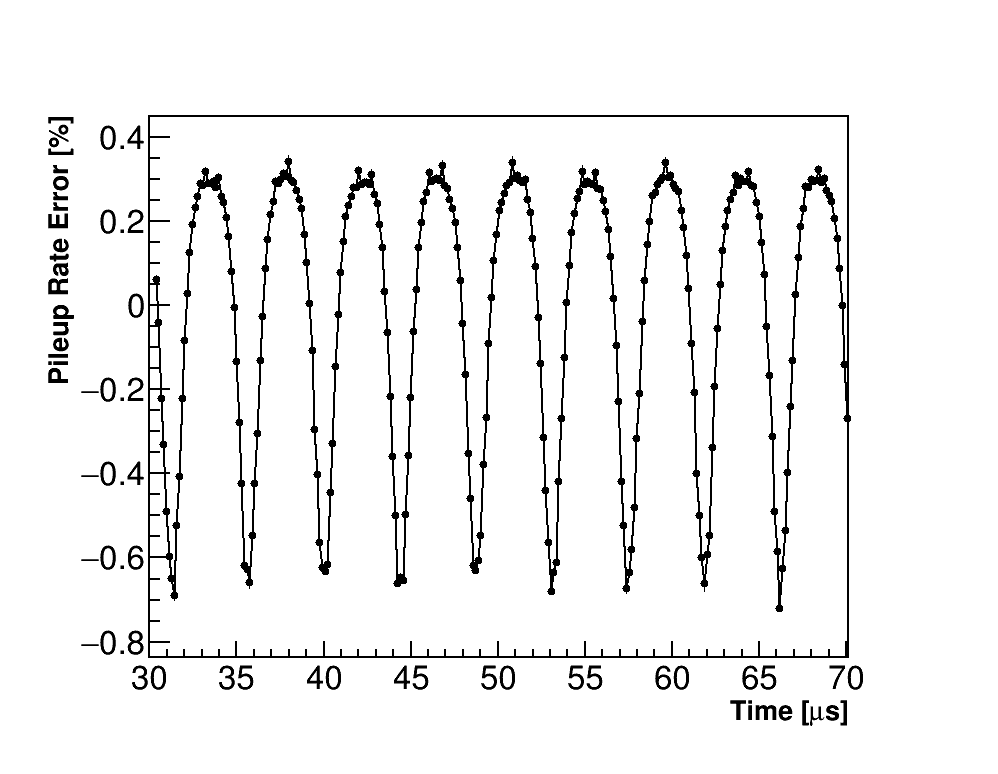
\includegraphics[width=.6\textwidth]{PileupRateError_149p2SGT}
    \caption[]{Pileup rate uncertainty when using a gap time of \SI{149.2}{\ns}. Data are from the 60h dataset.}
    \label{fig:pileupRateErrorLarger}
\end{figure}




\clearpage
\subsection{Unseen Pileup}

A systematic uncertainty arises due to unseen pileup, from those counts with energies smaller than the threshold of the detector systems, which is typically around 50~\MeV. These unseen pulses do not get reconstructed as clusters, but will still contribute to pileup if they hit the detectors at the same time as higher energy pulses. A conservative bound of this effect on \R can be calculated by constructing the pileup such that it ignores pulses below \SI{100}{\MeV}, a value which is twice as high as the expected missed pulse energies. The systematic uncertainties, taken as the \DR values with this alternate procedure in place, are given in \tabref{tab:systematicError_unseenPileup}. If instead the threshold is raised to \SI{200}{\MeV} then the systematic uncertainties range approximately from 10-30 ppb.


\begin{table}[h]
\centering
\renewcommand{\arraystretch}{1.2}
\begin{tabularx}{0.6\linewidth}{@{\extracolsep{\fill}}XYY}
  \hline
    \multicolumn{3}{c}{\textbf{Unseen Pileup Systematic Uncertainty}} \\
  \hline\hline
    Dataset & \thead{T-Method} & \thead{R-Method} \\
  \hline
    60h & 0.8 & 0.6 \\
    HighKick & 1.3 & 0.1 \\
    9d & 2.5 & 2.5 \\ 
    Endgame & 4.1 & 2.4 \\
  \hline
\end{tabularx}
\caption[]{Systematic uncertainty due to unseen pileup. Units are in ppb.}
\label{tab:systematicError_unseenPileup}
\end{table}



\clearpage
\subsection{Triple Pileup Correction}

Triple pileup is not included in the pileup correction, and therefore introduces a systematic uncertainty. The systematic uncertainty for ignoring the triples is estimated by looking at the $\Delta R$ with and without the doubles correction, multiplied against the rate of triples to doubles. The former can be determined from the slopes of the pileup multiplier scans extrapolated to 0, \tabref{tab:pileupMultplierScan}, while the latter can be approximated by the rate of doubles to singles, \figref{fig:pileupRateFraction}. As shown the fraction of pileup is less than 1\% and decreases throughout the fill. For a conservative approach, the rate is averaged over the first \gmtwo period before multiplying against the \DR value with and without the doubles correction. These rate values are given in \tabref{tab:pileupRates}, along with the maximum rates in the same period. The systematic uncertainties are given in \tabref{tab:systematicError_triplePileupCorrection}. As shown the systematic uncertainties are $\mathcal{O}(1)$~ppb, and even these small numbers are conservative since the rate drops throughout the fill, and would drop even faster for triples to doubles.


\begin{figure}[h]
    \centering
    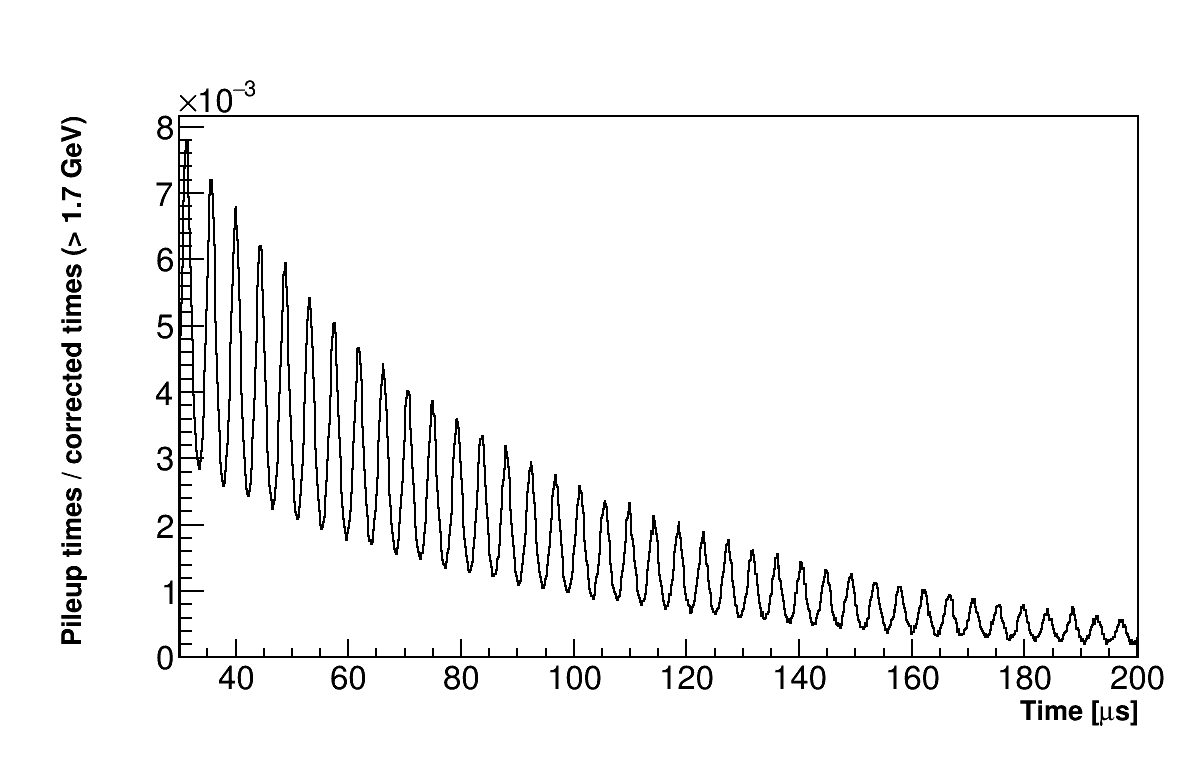
\includegraphics[width=0.6\textwidth]{pileupRateFraction}
    \caption[]{Pileup rate fraction plot. Data from the Endgame dataset.}
    \label{fig:pileupRateFraction}
\end{figure}


\begin{table}[h]
\centering
\renewcommand{\arraystretch}{1.2}
\begin{tabularx}{0.5\linewidth}{@{\extracolsep{\fill}}lcc}
  \hline
    \multicolumn{3}{c}{\textbf{Pileup Rates}} \\
  \hline\hline
    Dataset & Average rate & Max rate \\
  \hline
    60h & \num{5.33e-3} & \num{8.50e-3} \\
    HighKick & \num{5.69e-3} & \num{8.96e-3} \\
    9d & \num{5.19e-3} & \num{8.32e-3} \\ 
    Endgame & \num{4.93e-3} & \num{7.78e-3} \\
  \hline
\end{tabularx}
\caption[]{Pileup rates over the first \gmtwo period of the fitting range, averaged and the maximum value respectively.}
\label{tab:pileupRates}
\end{table}


\begin{table}[h]
\centering
\renewcommand{\arraystretch}{1.2}
\begin{tabularx}{0.5\linewidth}{@{\extracolsep{\fill}}XYY}
  \hline
    \multicolumn{3}{c}{\textbf{Triple Pileup Systematic Uncertainty}} \\
  \hline\hline
    Dataset & \thead{T-Method} & \thead{R-Method} \\
  \hline
    60h & 1.9 & 1.6 \\
    HighKick & 1.3 & 1.2 \\
    9d & 1.0 & 1.1 \\ 
    Endgame & 1.6 & 1.3 \\
  \hline
\end{tabularx}
\caption[]{Systematic uncertainty due to triple pileup correction. Units are in ppb.}
\label{tab:systematicError_triplePileupCorrection}
\end{table}




%!TEX root = ../BUSystematics.tex

\graphicspath{{Body/Figures/MuonLosses/}}

\section{Muon Loss Systematic Errors}

\subsection{Time Cuts}

\subsection{Energy Cuts}

\subsection{Muon Loss Scale Fixed}

%!TEX root = ../BUSystematics.tex

\graphicspath{{Body/Figures/CBO/}{Body/Figures/CBO/Frequency/}{Body/Figures/CBO/TimeConstants/}}

\clearpage
\section{CBO Systematic Uncertainties}

\subsection{Frequency Change}


The systematic error due to the fixed CBO frequency model is calculated as the \DR with the Tracker Station 12 vs Tracker Station 18 parameters. These parameters are given in \refref{CBOFreqTrackingElog}, and the Endgame parameters are shown in \figref{fig:CBOFreq}. \tabref{tab:systematicError_CBOFreq} gives the systematic errors.

The HighKick and 9d Ratio results are less affected, presumably because the lifetime is fixed in those fits and there is a correlation.


\begin{figure}[h]
    \centering
    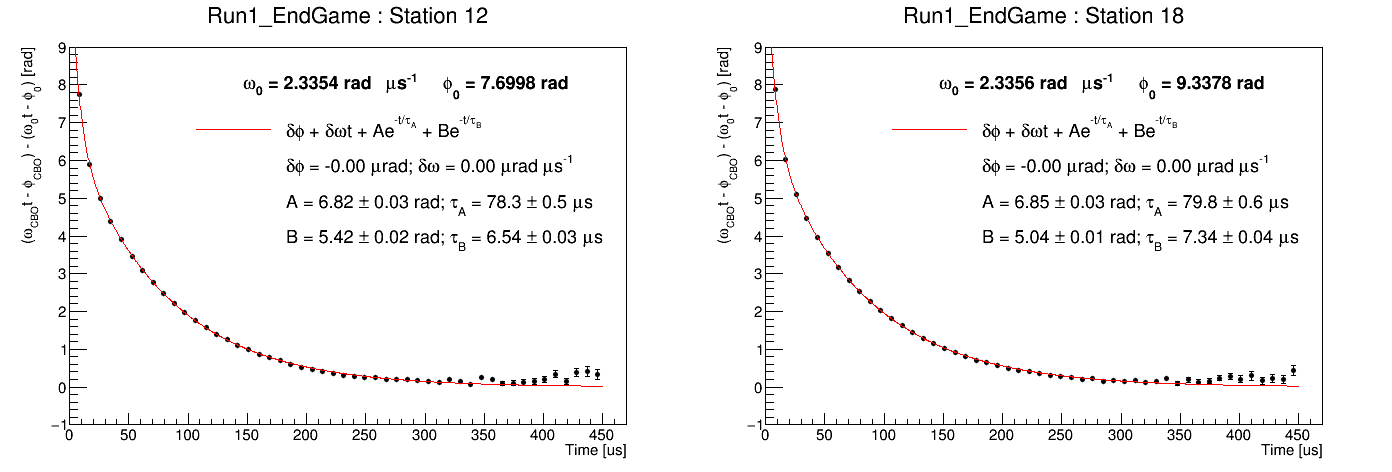
\includegraphics[width=\textwidth]{Run1_EndGame_CBOFreq}
    \caption[]{CBO frequency parameters for the Endgame dataset as determined in the tracking analysis. The y axis is in units of ... (see thesis description)}
    \label{fig:CBOFreq}
\end{figure}


\begin{table}[h]
\centering
\renewcommand{\arraystretch}{1.2}
\begin{tabularx}{0.65\linewidth}{@{\extracolsep{\fill}}XYY}
  \hline
    \multicolumn{3}{c}{\textbf{Systematic Error due to CBO Frequency}} \\
  \hline\hline
    Dataset & \thead{T-Method} & \thead{R-Method} \\
  \hline
    60h & 10.9 & 5.3 \\
    HighKick & 22.5 & 0.7 \\
    9d & 21.3 & 1.6 \\ 
    Endgame & 22.2 & 8.5 \\
  \hline
\end{tabularx}
\caption[Systematic error due to CBO frequency]{Systematic error due to CBO frequency. Units are in ppb.}
\label{tab:systematicError_CBOFreq}
\end{table}




\clearpage
\subsection{Decoherence Envelope}


The systematic error from the CBO decoherence envelope was estimated by introducing a constant $C$ in the CBO function part of the fit equation and then looking at the \DR. This constant was allowed to float...


might want to include figure of amplitude shape like in thesis showing the C constant is a reasonable adjustment

\begin{table}[h]
\centering
\setlength\tabcolsep{10pt}
\renewcommand{\arraystretch}{1.2}
\begin{tabularx}{0.6\linewidth}{XYYY}
  \hline
    \multicolumn{4}{c}{\textbf{Fitted CBO envelope constants}} \\
  \hline\hline
    Dataset & \thead{Fit Method} & \multicolumn{1}{c}{$C$} & \multicolumn{1}{c}{$\delta C$} \\
  \hline
    \multirow{2}{*}{60h} & \thead{T} & 7.1 & 4.0 \\
                         & \thead{R} & 16.1 & 5.1 \\
  \hline
    \multirow{2}{*}{HighKick} & \thead{T} & 5.2 & 1.8 \\
                              & \thead{R} & 15.7 & 11.2 \\
  \hline
    \multirow{2}{*}{9d} & \thead{T} & 7.8 & 2.9 \\
                        & \thead{R} & 13.7 & 12.3 \\
  \hline
    \multirow{2}{*}{Endgame} & \thead{T} & 5.5 & 2.1 \\
                             & \thead{R} & 10.9 & 3.4 \\
  \hline
    \multirow{2}{*}{Endgame at \mus{50}} & \thead{T} & 4.7 & 2.6 \\
                                         & \thead{R} & 9.0 & 4.5 \\
  \hline  
\end{tabularx}
\caption[]{Units are in 1e-4.}
\label{tab:CBOenvConstants}
\end{table}





\begin{table}
\centering
\renewcommand{\arraystretch}{1.2}
\begin{tabularx}{\linewidth}{@{\extracolsep{\fill}}XYY}
  \hline
    \multicolumn{3}{c}{\textbf{Systematic Error due to CBO Decoherence Envelope}} \\
  \hline\hline
    Dataset & \thead{T-Method} & \thead{R-Method} \\
  \hline
    60h & 38.3 & 5.5 \\
    HighKick & 3.7 & 9.1 \\
    9d & 13.4 & 0.2 \\ 
    Endgame & 3.3 & 5.9 \\
    Endgame at \mus{50} & 25.3 & 18.0 \\
  \hline
\end{tabularx}
\caption[Systematic error due to CBO decoherence envelope]{Systematic error due to CBO decoherence envelope. Units are in ppb.}
\label{tab:systematicError_CBOenvelope}
\end{table}



\clearpage
\subsection{Time Constants}

In the fit function the N, asymmetry, and phase terms all have CBO modifications to them, where there are new cbo amplitude and phase paramters for each parameter. The lifetime is typically fixed to be the same in all cases. However it has been claimed that the CBO lifetime on the asymmetry and phase CBO terms could be as much as 50\% different from that of the N term. In order to evaluate a systematic error due to this possibility, fits were redone by applying multipliers of 0.5 and 1.5 in the various combinations to the respective lifetimes, for a total of 4 new fits for each dataset. The maximum \DR seen from any of the combinations was then taken as the systematic error on \R. Typically the combinations of 0.5 and 1.5 produced the largest changes, as opposed to both being 0.5 or 1.5.



\begin{table}
\centering
\setlength\tabcolsep{10pt}
\renewcommand{\arraystretch}{1.2}
\begin{tabularx}{\linewidth}{@{\extracolsep{\fill}}lGGGG}
  \hline
    \multicolumn{5}{c}{\textbf{T-Method \DR with multipliers on CBO asymmetry and phase lifetimes}} \\
  \hline\hline
    Dataset & \thead{(0.5, 0.5)} & \thead{(1.5, 0.5)} & \thead{(0.5, 1.5)} & \thead{(1.5, 1.5)} \\
  \hline
    60h & -6.3 & 8.6 & \multicolumn{1}{K}{-10.8} & 4.3 \\
    HighKick & -9.6 & \multicolumn{1}{K}{23.1} & -22.7 & 9.8 \\
    9d & 15.7 & -13.0 & \multicolumn{1}{K}{23.4} & -5.7 \\ 
    Endgame & -8.2 & 5.4 & \multicolumn{1}{K}{-10.5} & 3.2 \\
  \hline
\end{tabularx}
\caption[]{\DR's for the various multiplier combinations for the T-Method fits. Multipliers are on the asymmetry and phase CBO lifetime respectively. The absolute value of the bold elements are taken as the systematic errors for the various datasets. Units are in ppb.}
\label{tab:systematicError_}
\end{table}


\begin{table}
\centering
\setlength\tabcolsep{10pt}
\renewcommand{\arraystretch}{1.2}
\begin{tabularx}{\linewidth}{@{\extracolsep{\fill}}lGGGG}
  \hline
    \multicolumn{5}{c}{\textbf{R-Method \DR with multipliers on CBO asymmetry and phase lifetimes}} \\
  \hline\hline
    Dataset & \thead{(0.5, 0.5)} & \thead{(1.5, 0.5)} & \thead{(0.5, 1.5)} & \thead{(1.5, 1.5)} \\
  \hline
    60h & -0.1 & 9.3 & \multicolumn{1}{K}{-10.8} & -1.8 \\
    HighKick & -13.1 & 18.0 & \multicolumn{1}{K}{-21.8} & 9.3 \\
    9d & -2.4 & -28.7 & \multicolumn{1}{K}{30.9} & 3.3 \\ 
    Endgame & -6.9 & 5.0 & \multicolumn{1}{K}{-9.8} & 2.3 \\
  \hline
\end{tabularx}
\caption[]{\DR's for the various multiplier combinations for the R-Method fits. Multipliers are on the asymmetry and phase CBO lifetime respectively. The absolute value of the bold elements are taken as the systematic errors for the various datasets. Units are in ppb.}
\label{tab:systematicError_}
\end{table}





\clearpage
\subsection{Time Constants Fixed}

In the HighKick and 9d datasets the CBO lifetimes in the R-Method fits are fixed to those from corresponding T-Method fits, since otherwise the fits do not like to converge to a nice value. In order to determine a systematic error from this fixed parameter, the sensitivity of \R to this fixed parameter was determined, and then multiplied against the T-Method fit error on the parameter. The scans are shown in \figref{fig:CBOfixedLifetime}. The scan results and systematic error are shown in \tabref{tab:systematicError_FixedCBOLifetime}.



\begin{figure}[h]
\centering
    \begin{subfigure}[t]{0.45\textwidth}
        \centering
        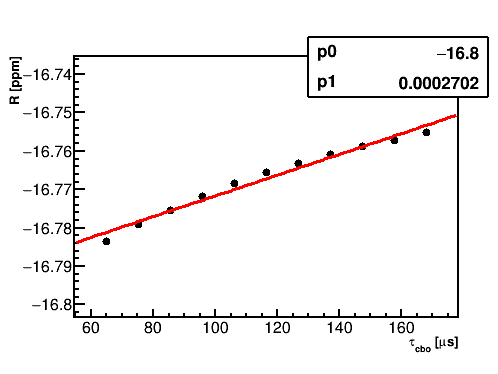
\includegraphics[width=\textwidth]{FullRatio_R_Vs_tau_cbo_Canv_HK}
        \caption{HighKick dataset.}
    \end{subfigure}% %you need this % here to add spacing between subfigures
    \hspace{1cm}
    \begin{subfigure}[t]{0.45\textwidth}
        \centering
        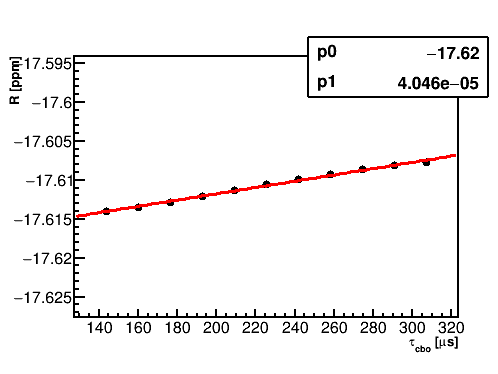
\includegraphics[width=\textwidth]{FullRatio_R_Vs_tau_cbo_Canv_9d}
        \caption{9d dataset.}
    \end{subfigure}
\caption[]{\R vs fixed CBO lifetime. The parameter $p_{1}$ is in units of ppm/microseconds.}
\label{fig:CBOfixedLifetime}
\end{figure}


\begin{table}
\centering
\renewcommand{\arraystretch}{1.2}
\begin{tabularx}{0.65\linewidth}{@{\extracolsep{\fill}}XccY}
  \hline
    \multicolumn{4}{c}{\textbf{Systematic Error due to fixed CBO lifetime}} \\
  \hline\hline
    Dataset & \thead{$dR/d\tau_{cbo}$} & \thead{T-Method $\sigma_{\tau_{cbo}}$} & \thead{R-Method \dR} \\
  \hline
    HighKick & 0.27 & 10.3 & 2.8 \\
    9d & 0.04 & 16.3 & 0.7 \\ 
  \hline
\end{tabularx}
\caption[Systematic error due to fixed CBO lifetime]{Systematic error due to fixed CBO lifetime. Units are in ppb for the error. Units are ppb per microsecond and microsecond for the other two quantities.}
\label{tab:systematicError_FixedCBOLifetime}
\end{table}

%!TEX root = ../BUSystematics.tex

\graphicspath{{Body/Figures/Ratio/}}

\section{Ratio Construction Systematic Errors}

In the Ratio Method the \gmtwo period and the muon lifetime are taken to be known a priori. If the parameters are incorrectly chosen then it is possible there will be a systematic shift on \R. See Section 5.5.5 in \refref{phdthesis:2020Kinnaird} for a full description of the techniques used to estimate the sensitivities of \R to these two parameters, and the expected uncertainties in the parameters. The uncertainties on the period and lifetime are \SI{21.7}{ppm} and \SI{<10}{ns} respectively, and the sensitivities in the various datasets are given in \tabref{tab:ratioConstructionParsScan}. Multiplying the sensitivities to the \gmtwo period by the uncertainty, the systematic errors are 0.7, 2.3, 0.9, and \ppb{1.0} for the 60h, HighKick, 9d, and Endgame datasets respectively. Since there is no reason the datasets should treat this parameter differently, the largest number at 2.3 ppb is taken as the sysetmatic error for all datasets. Regarding the systematic error for the choice of muon lifetime, the slopes are so small and the error on the lifetime is so small such that the systematic error is completely negligible, and is taken to be 0 for all datasets.



\begin{table}
\centering
\setlength\tabcolsep{20pt}
\renewcommand{\arraystretch}{1.2}
\begin{tabular*}{0.7\linewidth}{@{\extracolsep{\fill}}lcHH}
  \hline
    \multicolumn{4}{c}{\textbf{Sensitivity to Ratio Construction Parameters}} \\
  \hline\hline
    Dataset & & \multicolumn{1}{c}{$dR/d_{T_{a}}$} & \multicolumn{1}{c}{$dR/d_{\tau_{\mu}}$} \\
  \hline
    60h & & 0.034 & -1.336 \\
    HighKick & & -0.105 & -5.914 \\
    9d & & 0.042 & 0.546 \\ 
    Endgame & & 0.044 & 1.705 \\
  \hline
\end{tabular*}
\caption[Sensitivities of $R$ to ratio construction parameters]{Sensitivities of $R$ to ratio construction parameters. $dR/d_{T_{a}}$ is in units of ppb/ppm, while $dR/d_{\tau_{\mu}}$ is in units of \SI{}{ppb/ \micro s}. In both cases the sensitivities are extremely small.}
\label{tab:ratioConstructionParsScan}
\end{table}




%!TEX root = ../BUSystematics.tex

\section{Conclusions}



Include total error table here of just my errors (not everybody elses)

- probably include one line which is the error if all the errors were uncorrelated

- include a reference to David's combination note \cite{CombinationNote} - Table 3 
- potentially include a reference to the uncertainty spreadsheet \cite{UncertaintySpreadsheet}




% notes: Need to decide what to do about errors that are not calculated in my own analysis but which apply as an error.
% Should probably include the actual numbers in this document as well in the form of tables for each dataset.




%==========================================================================%
% Bibliography
% \newpage
\addcontentsline{toc}{section}{References}
\printbibliography

%==========================================================================%
\end{document}
